\chapter{线性偏微分方程}


\vspace{-2em}
本章旨在说明如何将泛函分析的抽象技巧应用于椭圆型、抛物型和双曲型偏微分方程的求解.

线性椭圆型方程由一个二阶微分算子定义，该算子是线性的但无界.因此，第一步须给出边值问题的一种替代性“弱”表述，其中涉及有界线性算子.

在某些情形下，可在Hilbert-Soblev空间 ${H}_{0}^{1}$ 上对一个适当的双线性型应用Lax-Milgram定理，得到唯一解.更一般的情形可借助Fredholm理论在${L}^{2}$中研究.当算子自伴时，由Hilbert-Schmidt定理，我们将以一组正交的特征函数级数来表示解.

抛物型与双曲型演化方程将通过线性半群理论加以研究.当定义算子为自伴时，解亦可表示为特征函数级数之和.

\section{椭圆型方程}

设 $\Omega  \subset  {\mathbb{R}}^{n}$ 为一有界开集.给定可测函数 ${a}^{ij},{b}^{i},c$ : $\Omega  \mapsto  \mathbb{R}$ ，考虑如下线性二阶微分算子
\begin{equation}\tag{9.1}\label{eq:linpde-9-1}
{Lu} \doteq   - \sum_{{i,j = 1}}^{n}{\left( {a}^{ij}\left( x\right) {u}_{{x}_{i}}\right) }_{{x}_{j}} + \sum_{{i = 1}}^{n}{\left( {b}^{i}\left( x\right) u\right) }_{{x}_{i}} + c\left( x\right) u.
\end{equation}

我们将研究边值问题的解
\begin{equation}\tag{9.2}\label{eq:linpde-9-2}
\begin{cases} {Lu}  = f, & x \in  \Omega , \\  u  = 0, & x \in  \partial \Omega , \end{cases}
\end{equation}
其中 $f \in  {L}^{2}\left( \Omega \right)$ 为给定函数.要求 $u$ 沿 $\partial \Omega$ 为零，称为\bluebf{Dirichlet边界条件}.

为便于后续参考，我们汇总本章通篇所用的主要假设.

(H) 定义域 $\Omega  \subset  {\mathbb{R}}^{n}$ 是开且有界的.算子\eqref{eq:linpde-9-1}中 $L$ 的系数满足
\begin{equation}\tag{9.3}\label{eq:linpde-9-3}
{a}^{ij},{b}^{i},c \in  {L}^{\infty }\left( \Omega \right) .
\end{equation}

此外，算子 $L$ 是一致椭圆的，即存在常数 $\theta  > 0$ ，使得
\begin{equation}\tag{9.4}\label{eq:linpde-9-4}
\sum_{{i,j = 1}}^{n}{a}^{ij}\left( x\right) {\xi }_{i}{\xi }_{j} \geq  \theta {\left| \xi \right| }^{2}\;\forall\,x \in  \Omega ,\xi  \in  {\mathbb{R}}^{n}.
\end{equation}

\begin{remark}\label{rem:linpde-9-1}
依定义，算子 $L$ 的一致椭圆性仅依赖于系数 ${a}^{ij}$ .在对称情形 ${a}^{ij} = {a}^{ji}$ 下，上述条件意味着:对每个 $x \in  \Omega$ ， $n \times  n$ 阶对称矩阵 $A\left( x\right)  = \left( {{a}^{ij}\left( x\right) }\right)$ 严格正定，且其最小特征值为 $\geq  \theta$ .
\end{remark}


\subsection{物理诠释}
举例而言，考虑流体以速度 $\bm{b}\left( x\right)  = \left( {{b}^{1},{b}^{2},{b}^{3}}\right) \left( x\right)$ 在区域 $\Omega  \subset  {\mathbb{R}}^{3}$ 内运动，设 $u = u\left( {t,x}\right)$ 描述分散于该流体中的某种化学物质的密度.

对任意子区域 $V \subset  \Omega$ ，假定 $V$ 内所含化学物质的总量仅因经边界 $\partial V$ 流入或流出的通量而改变，即
\begin{equation}\tag{9.5}\label{eq:linpde-9-5}
\frac{d}{\d t}{\int }_{V}{u\d x} = {\int }_{\partial V}\bm{n} \cdot  \left( {a\nabla u}\right) {dS} - {\int }_{\partial V}\bm{n} \cdot  \left( {\bm{b}u}\right) {dS}.
\end{equation}

此处 $\bm{n}\left( x\right)$ 表示集合 $V$ 在边界点 $x$ 处的单位外法向量，而 $a > 0$ 为常数扩散系数.式\eqref{eq:linpde-9-5}右端第一项积分描述了化学物质经扩散穿过边界进入的量；注意，当 $\bm{n} \cdot  \nabla u > 0$ 时该项为正.这发生在区域 $V$ 外部的化学物质浓度高于内部的情形.第二项积分(带负号)则表示化学物质经对流穿过 $V$ 边界向外迁移的量，即被运动流体携带输送(图\ref{fig:linpde-9-1-1}).
\begin{figure}[htbp]
    \vspace{-1em}
\centering
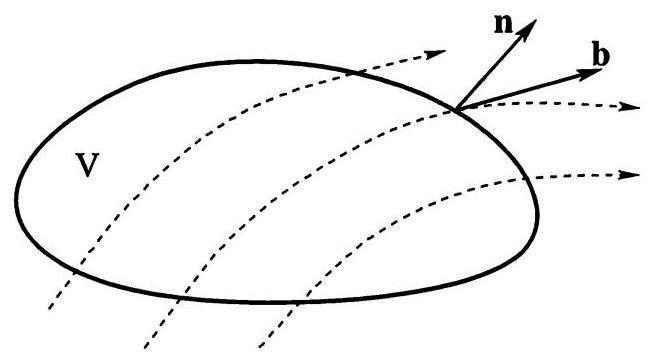
\includegraphics[width=0.6\textwidth]{images/bo_d6ik6nn7aajc739ct1l0_199_417_243_649_359_0.jpg}
\caption{化学物质穿过 $V$ 边界输运时，$V$ 内部所含总量随时间变化.}
\label{fig:linpde-9-1-1}
\end{figure}

利用散度定理，由\eqref{eq:linpde-9-5}可得
\begin{equation}\tag{9.6}\label{eq:linpde-9-6}
{\int }_{V}{u}_{t}{\d x} = {\int }_{V}{a\Delta u\d x} - {\int }_{V}\operatorname{div}\left( {\bm{b}u}\right) {\d x}.
\end{equation}

由于上述恒等式在每个子区域 $V \subset  \Omega$ 上均成立，我们得出 $u = u\left( {t,x}\right)$ 满足抛物型偏微分方程
\[\begin{matrix}
    &{u}_{t}& - &{a\Delta u}&+ &\operatorname{div}\left( {\bm{b}u}\right)&  = &0.\\
    & & & \text{ [扩散]}& & \text{[对流] }& &
\end{matrix}\]


更一般的模型可描述以下情形:

\begin{itemize}\relax
\item\relax 扩散在整个区域上并非均匀:即系数 $a$ 不是常数，而是依赖于位置 $x \in  \Omega$ ；此外，扩散亦非各向同性——在某些方向上比其他方向更快.所有这些可通过将常数扩散矩阵 $A\left( x\right)  \equiv  {aI}$ 替换为更一般的对称矩阵 $A\left( x\right)  = \left( {{a}^{ij}\left( x\right) }\right)$ 来建模.
\end{itemize}

\begin{itemize}\relax
\item\relax $u$ 的总量并不守恒:存在额外项，分别对应线性衰减与外部源.
\end{itemize}

在 $n$ 维空间中，这导出如下形式的线性演化方程\eqref{eq:linpde-9-7}
\begin{equation}\tag{9.7}\label{eq:linpde-9-7}
\begin{matrix} {u}_{t} &  - & \sum_{{i,j = 1}}^{n}{\left( {a}^{ij}\left( x\right) {u}_{{x}_{i}}\right) }_{{x}_{j}} &  + & \sum_{{i = 1}}^{n}{\left( {b}^{i}\left( x\right) u\right) }_{{x}_{i}} &  = &  - c\left( x\right) u &  + & f\left( x\right) \;. \\   & & \text{ [扩散] } & & \text{ [衰减] } & & \text{ [衰减] } & & \text{ [衰减] } \end{matrix}
\end{equation}

方程\eqref{eq:linpde-9-7}可用于建模多种现象，例如质量输运、热传导等.在许多情况下，人们关注稳态解，即与时间无关的解.在\eqref{eq:linpde-9-7}中令 ${u}_{t} = 0$ ，可得线性椭圆型方程
\begin{equation}\tag{9.8}\label{eq:linpde-9-8}
- \sum_{{i,j = 1}}^{n}{\left( {a}^{ij}\left( x\right) {u}_{{x}_{i}}\right) }_{{x}_{j}} + \sum_{{i = 1}}^{n}{\left( {b}^{i}\left( x\right) u\right) }_{{x}_{i}} + c\left( x\right) u = f\left( x\right) .
\end{equation}

\subsection{经典解与弱解}
边界值问题\eqref{eq:linpde-9-2}的经典解是指一个函数 $u \in  {\mathcal{C}}^{2}\left( \Omega \right)$ ，它在每一点均满足方程及边界条件.一般而言，由于方程系数缺乏正则性，问题\eqref{eq:linpde-9-2}可能不存在经典解，因此需引入更弱的解的概念.

\begin{definition}\label{def:linpde-9-2}
\eqref{eq:linpde-9-2}的弱解是一个函数 $u \in  {H}_{0}^{1}\left( \Omega \right)$ ，使得
\begin{equation}\tag{9.9}\label{eq:linpde-9-9}
{\int }_{\Omega }\left( {\sum_{{i,j = 1}}^{n}{a}^{ij}{u}_{{x}_{i}}{v}_{{x}_{j}} - \sum_{{i = 1}}^{n}{b}^{i}u{v}_{{x}_{i}} + {cuv}}\right) {\d x} = {\int }_{\Omega }{fv\d x},\;\forall\,v \in  {H}_{0}^{1}\left( \Omega \right) .
\end{equation}
\end{definition}

\begin{remark}\label{rem:linpde-9-3}
边界条件 $u = 0$ 在 $\partial \Omega$ 上通过要求 $u \in  {H}_{0}^{1}\left( \Omega \right)$ 得以体现.\eqref{eq:linpde-9-9}式形式上由下式经分部积分得到
\begin{equation}\tag{9.10}\label{eq:linpde-9-10}
{\int }_{\Omega }\left( {Lu}\right) {v\d x} = {\int }_{\Omega }{fv\d x}\;\forall\,v \in  {\mathcal{C}}_{c}^{\infty }\left( \Omega \right)
\end{equation}
并分部积分.注意，若\eqref{eq:linpde-9-9}对任意检验函数 $v \in  {\mathcal{C}}_{c}^{\infty }\left( \Omega \right)$ 成立，则通过逼近论证，该积分恒等式对任意 $v \in  {H}_{0}^{1}\left( \Omega \right)$ 仍成立.须特别指出的是，函数 $u \in  {H}_{0}^{1}$ 可能不具有二阶弱导数；但\eqref{eq:linpde-9-9}中的积分对所有 $u,v \in  {H}_{0}^{1}$ 始终良定.
\end{remark}

弱解概念的一种便捷重述方式如下:在Hilbert空间 ${H}_{0}^{1}\left( \Omega \right)$ 上，考虑双线性型
\begin{equation}\tag{9.11}\label{eq:linpde-9-11}
B\left(  {u,v}\right)   \doteq  {\int }_{\Omega }\left( {\sum_{{i,j = 1}}^{n}{a}^{ij}{u}_{{x}_{i}}{v}_{{x}_{j}} - \sum_{{i = 1}}^{n}{b}^{i}u{v}_{{x}_{i}} + {cuv}}\right) {\d x}.
\end{equation}

函数 $u \in  {H}_{0}^{1}$ 是\eqref{eq:linpde-9-2}的弱解，当且仅当
\begin{equation}\tag{9.12}\label{eq:linpde-9-12}
B\left(  {u,v}\right)   = {\left( f,v\right) }_{{L}^{2}},\;\forall\,v \in  {H}_{0}^{1}.
\end{equation}

此处及后文，我们采用记号
\begin{equation}\tag{9.13}\label{eq:linpde-9-13}
{\left( f,g\right) }_{{L}^{2}} \doteq  {\int }_{\Omega }{fg\d x}
\end{equation}
表示 ${L}^{2}\left( \Omega \right)$ 中的内积，以区别于 ${H}^{1}\left( \Omega \right)$ 中的内积
\begin{equation}\tag{9.14}\label{eq:linpde-9-14}
{\left( f,g\right) }_{{H}^{1}} \doteq  {\int }_{\Omega }{fg\d x} + {\int }_{\Omega }\sum_{{i = 1}}^{n}{f}_{{x}_{i}}{g}_{{x}_{i}}{\d x}.
\end{equation}

\begin{remark}\label{rem:linpde-9-4}
方程\eqref{eq:linpde-9-1}中二阶项前的负号，在经形式分部积分后，在\eqref{eq:linpde-9-11}中消失.

后文将明确表明，该符号之选取旨在使相应二次型 $B\left(  {u,v}\right)$ 可为正定.
\end{remark}

\begin{remark}\label{rem:linpde-9-5}
给定函数 $g \in \; {H}^{1}\left( \Omega \right)$ ，可考虑非齐次边值问题
\begin{equation}\tag{9.15}\label{eq:linpde-9-15}
\begin{cases} {Lu} = f,  & x \in  \Omega , \\  u = g, & x \in  \partial \Omega . \end{cases}
\end{equation}

该问题可重写为关于函数 $\widetilde{u} \doteq  u - g$ 的齐次问题，即
\begin{equation}\tag{9.16}\label{eq:linpde-9-16}
\begin{cases} L\widetilde{u} = f - {Lg}, & x \in  \Omega , \\  \widetilde{u} = 0, & x \in  \partial \Omega . \end{cases}
\end{equation}

假设 ${Lg} \in  {L}^{2}\left( \Omega \right)$ ，则问题\eqref{eq:linpde-9-16}与\eqref{eq:linpde-9-2}完全属于同一类型.
\end{remark}

\begin{remark}\label{rem:linpde-9-6}
形如
\[
{Lu} \doteq   - \sum_{{i,j = 1}}^{n}{a}^{ij}\left( x\right) {u}_{{x}_{i}{x}_{j}} + \sum_{{i = 1}}^{n}{b}^{i}\left( x\right) {u}_{{x}_{i}} + c\left( x\right) u
\]
的微分算子可重写为
\[
{Lu} =  - \sum_{{i,j = 1}}^{n}{\left( {a}^{ij}\left( x\right) {u}_{{x}_{i}}\right) }_{{x}_{j}} + \sum_{{i = 1}}^{n}\left( {{b}^{i}\left( x\right)  + \sum_{{j = 1}}^{n}{a}^{ij}{}_{{x}_{j}}\left( x\right) }\right) {u}_{{x}_{i}} + c\left( x\right) u.
\]

假设 ${a}^{ij},{a}^{ij}{}_{{x}_{j}},{b}^{i},c \in  {L}^{\infty }\left( \Omega \right)$ ，相应问题\eqref{eq:linpde-9-2}的弱解仍可通过求解\eqref{eq:linpde-9-12}得到，其中双线性型 $B$ 现定义为
\[
B\left(  {u,v}\right)   \doteq  {\int }_{\Omega }\left( {\sum_{{i,j = 1}}^{n}{a}^{ij}{u}_{{x}_{i}}{v}_{{x}_{j}} + \sum_{{i = 1}}^{n}\left( {{b}^{i} + \sum_{{j = 1}}^{n}{a}^{ij}}\right) {u}_{{x}_{i}}v + {cuv}}\right) {\d x}.
\]
\end{remark}

作为第一个例子，考虑边值问题
\begin{equation}\tag{9.17}\label{eq:linpde-9-17}
\begin{cases}  - {\Delta u} + u   = f, & x \in  \Omega , \\[-3pt]  u  = 0, & x \in  \partial \Omega . \end{cases}
\end{equation}

显然，算子 $- {\Delta u} \doteq   - \sum_{i}{u}_{{x}_{i}{x}_{i}}$ 是一致椭圆的，因为此时 $n \times  n$ 矩阵 $A\left( x\right)  = \left( {{a}^{ij}\left( x\right) }\right)$ 对每个 $x \in  \Omega$ 均为单位矩阵.问题\eqref{eq:linpde-9-17}弱解的存在性可通过基于Riesz表示定理的一个极为简洁的论证予以证明.

\begin{lemma}\label{lem:linpde-9-7}
设 $\Omega  \subset  {\mathbb{R}}^{n}$ 为有界开集.则对任意 $f \in  {L}^{2}\left( \Omega \right)$ ，边值问题\eqref{eq:linpde-9-17}存在唯一弱解 $u \in  {H}_{0}^{1}\left( \Omega \right)$ .相应的映射 $f \mapsto  u$ 是从 ${L}^{2}\left( \Omega \right)$ 到 ${H}_{0}^{1}\left( \Omega \right)$ 的紧线性算子.
\end{lemma}

\begin{proof}
由Rellich-Kondrachov定理，标准嵌入 $\iota$ : ${H}_{0}^{1}\left( \Omega \right)  \mapsto  {L}^{2}\left( \Omega \right)$ 是紧的.故其对偶算子 ${\iota }^{ * }$为紧算子.由于 ${H}_{0}^{1}$ 与 ${L}^{2}$ 均为Hilbert空间，故可与其对偶空间恒等.由此得到:
\begin{equation}\tag{9.18}\label{eq:linpde-9-18}
\setjot[-2]\begin{aligned}
{H}_{0}^{1}\left( \Omega \right) &\overset{\iota }{ \rightarrow  }{L}^{2}\left( \Omega \right)\\
{H}_{0}^{1}\left( \Omega \right)  = {\left(  {H}_{0}^{1}\left( \Omega \right) \right)  }^{ * } &\overset{{\iota }^{ * }}{ \leftarrow  }{\left(  {L}^{2}\left( \Omega \right) \right)  }^{ * } = {L}^{2}\left( \Omega \right) .
\end{aligned}
\end{equation}

对每个 $f \in  {L}^{2}\left( \Omega \right)$ ，由对偶算子定义可得
\[
{\left( {\iota }^{ * }f,v\right) }_{{H}^{1}} = {\left( f,\iota v\right) }_{{L}^{2}} = {\left( f,v\right) }_{{L}^{2}}\;\forall\,f \in  {L}^{2}\left( \Omega \right) ,v \in  {H}_{0}^{1}\left( \Omega \right) .
\]

由\eqref{eq:linpde-9-14}可知， ${\iota }^{ * }f$ 恰为\eqref{eq:linpde-9-17}的弱解.
\end{proof}


\subsection{齐次二阶椭圆算子}
我们首先研究椭圆边值问题
\begin{equation}\tag{9.19}\label{eq:linpde-9-19}
\begin{cases} {Lu}  = f, & x \in  \Omega , \\[-3pt]  u = 0, & x \in  \partial \Omega , \end{cases}
\end{equation}
的解，其中微分算子 $L$ 仅含二阶项:
\begin{equation}\tag{9.20}\label{eq:linpde-9-20}
{Lu} \doteq   - \sum_{{i,j = 1}}^{n}{\left( {a}^{ij}\left( x\right) {u}_{{x}_{i}}\right) }_{{x}_{j}}.
\end{equation}

我们回顾:\eqref{eq:linpde-9-19}的弱解是指满足下式的函数 $u \in  {H}_{0}^{1}\left( \Omega \right)$
\begin{equation}\tag{9.21}\label{eq:linpde-9-21}
B\left(  {u,v}\right)   = {\left( f,v\right) }_{{L}^{2}}\;\forall\,v \in  {H}_{0}^{1}\left( \Omega \right) ,
\end{equation}
其中 $B : {H}_{0}^{1} \times  {H}_{0}^{1} \mapsto  \mathbb{R}$ 是连续双线性型
\begin{equation}\tag{9.22}\label{eq:linpde-9-22}
B\left(  {u,v}\right)   \doteq  {\int }_{\Omega }\sum_{{i,j = 1}}^{n}{a}^{ij}{u}_{{x}_{i}}{v}_{{x}_{j}}{\d x}.
\end{equation}

\begin{theorem}\label{thm:linpde-9-8}
设 $\Omega  \subset  {\mathbb{R}}^{n}$ 为有界开集.设\eqref{eq:linpde-9-20}中的算子 $L$ 一致椭圆，其系数为 ${a}^{ij} \in  {L}^{\infty }\left( \Omega \right)$ .则对任意 $f \in  {L}^{2}\left( \Omega \right)$ ，边值问题\eqref{eq:linpde-9-19}存在唯一弱解 $u \in  {H}_{0}^{1}\left( \Omega \right)$ .相应的解算子(记为 ${L}^{-1} : f \mapsto  u$ )是从 ${L}^{2}\left( \Omega \right)$ 到 ${H}_{0}^{1}\left( \Omega \right)$ 的紧线性算子.
\end{theorem}

\begin{proof}
椭圆边值问题\eqref{eq:linpde-9-19}弱解的存在性与唯一性，可通过验证双线性型 $B$ (见\eqref{eq:linpde-9-22})满足 Lax-Milgram 定理的所有条件而得到.

\noindent 1. $B$ 的连续性显然成立.事实上，
{\setjot[-2]\begin{align*}
    \left| {B\left(  {u,v}\right)  }\right|  &\leq  \sum_{{i,j = 1}}^{n}{\int }_{\Omega }\left| {{a}^{ij}{u}_{{x}_{i}}{v}_{{x}_{j}}}\right| {\d x} \leq  \sum_{{i,j = 1}}^{n}{\norm{a}^{ij}}_{{L}^{\infty }}{\norm{u}_{{x}_{i}}}_{{L}^{2}}{\norm{v}_{{x}_{j}}}_{{L}^{2}}\\
    &\leq  C\| u{\| }_{{H}^{1}}\| v{\| }_{{H}^{1}}
\end{align*}}

\noindent 2. 我们断言 $B$ 是严格正定的，即存在 $\beta  > 0$ ，使得
\begin{equation}\tag{9.23}\label{eq:linpde-9-23}
B\left(  {u,u}\right)  \; \geq  \;\beta \| u{\| }_{{H}^{1}\left( \Omega \right) }^{2}\;\forall\,u \in  {H}_{0}^{1}\left( \Omega \right) \;.
\end{equation}

事实上，由于 $\Omega$ 有界，Poincaré 不等式保证存在常数 $\kappa$ ，使得
\[
\| u{\| }_{{L}^{2}\left( \Omega \right) }^{2} \leq  \kappa {\int }_{\Omega }{\left| \nabla u\right| }^{2}{\d x}\;\forall\,u \in  {H}_{0}^{1}\left( \Omega \right) .
\]

另一方面，一致椭圆性条件蕴含
\[
B\left(  {u,u}\right)   = {\int }_{\Omega }\sum_{{i,j = 1}}^{n}{a}^{ij}{u}_{{x}_{i}}{u}_{{x}_{j}}{\d x} \geq  {\int }_{\Omega }\theta \sum_{{i = 1}}^{n}{u}_{{x}_{i}}^{2}{\d x} = \theta {\int }_{\Omega }{\left| \nabla u\right| }^{2}{\d x}.
\]

上述两个不等式联立可得
\[
\| u{\| }_{{H}^{1}}^{2} = \| u{\| }_{{L}^{2}}^{2} + \| \nabla u{\| }_{{L}^{2}}^{2} \leq  \left( {\kappa  + 1}\right) \| \nabla u{\| }_{{L}^{2}}^{2} \leq  \frac{\kappa  + 1}{\theta }B\left(  {u,u}\right)  .
\]

这证明了\eqref{eq:linpde-9-23}，其中 $\beta  = \theta /\left( {\kappa  + 1}\right)$ .

\noindent 3. 由 Lax-Milgram 定理，对任意 $\widetilde{f} \in  {H}_{0}^{1}\left( \Omega \right)$ ，存在唯一元素 $u \in  {H}_{0}^{1}$ ，使得
\begin{equation}\tag{9.24}\label{eq:linpde-9-24}
B\left(  {u,v}\right)   = {\left( \widetilde{f},v\right) }_{{H}^{1}}\;\forall\,v \in  {H}_{0}^{1}\left( \Omega \right) .
\end{equation}

此外，映射 $\Lambda  : \widetilde{f} \mapsto  u$ 连续，即
\[
\| u{\| }_{{H}^{1}} \leq  {\beta }^{-1}\| \widetilde{f}{\| }_{{H}^{1}}.
\]

取\eqref{eq:linpde-9-18}中定义的 $\widetilde{f} \doteq  {\iota }^{ * }f \in  {H}_{0}^{1}\left( \Omega \right)$ ，从而得到
\begin{equation}\tag{9.25}\label{eq:linpde-9-25}
B\left(  {u,v}\right)   = {\left( {\iota }^{ * }f,v\right) }_{{H}^{1}} = {\left( f,v\right) }_{{L}^{2}}\;\forall\,v \in  {H}_{0}^{1}\left( \Omega \right) .
\end{equation}

依定义， $u$ 是\eqref{eq:linpde-9-19}的弱解.

\noindent 4. 为证解算子 ${L}^{-1} : f \mapsto  u$ 是紧的，考虑如下图示
\[
{L}^{2}\left( \Omega \right) \overset{{\iota }^{ * }}{ \rightarrow  }{H}_{0}^{1}\left( \Omega \right) \overset{\Lambda }{ \rightarrow  }{H}_{0}^{1}\left( \Omega \right) .
\]

由引理\ref{lem:linpde-9-7}，线性算子${\iota }^{ * }$紧，且 $\Lambda$ 连续.因此复合算子${L}^{-1} = \Lambda  \circ  {\iota }^{ * }$ 是紧的.
\end{proof}

\subsection{按特征函数的展开表示}
由于 ${H}_{0}^{1}\left( \Omega \right)  \subset  {L}^{2}\left( \Omega \right)$ ，定理 9.8 所述的解算子 ${L}^{-1}$ 亦可视为从 ${L}^{2}\left( \Omega \right)$ 到其自身的紧算子.在对称情形 ${a}^{ij} = {a}^{ji}$ 下，算子 ${L}^{-1}$ 是自伴的.故由 Hilbert-Schmidt 定理，它可按一列可数的特征函数基展开表示.
\begin{theorem}\label{thm:linpde-9-9}
假设 ${a}^{ij} = {a}^{ji} \in  {L}^{\infty }\left( \Omega \right)$ .则在定理\ref{thm:linpde-9-8}的设定下，线性算子 ${L}^{-1} : {L}^{2}\left( \Omega \right)  \mapsto  {L}^{2}\left( \Omega \right)$ 是紧的、单射的且自伴的.

空间 ${L}^{2}\left( \Omega \right)$ 具有由 ${L}^{-1}$ 的特征函数构成的可数标准正交基 $\left\{  {{\phi }_{k};k \geq  1}\right\}$ ，且有如下表示
\begin{equation}\tag{9.26}\label{eq:linpde-9-26}
{L}^{-1}f = \sum_{{k = 1}}^{\infty }{\lambda }_{k}{\left( f,{\phi }_{k}\right) }_{{L}^{2}}{\phi }_{k}
\end{equation}
相应的特征值 ${\lambda }_{k}$ 满足
\begin{equation}\tag{9.27}\label{eq:linpde-9-27}
\mathop{\lim }\limits_{{k \rightarrow  \infty }}{\lambda }_{k} = 0,\;{\lambda }_{k} > 0\forall\,k \geq  1.
\end{equation}
\end{theorem}

\begin{proof}
1. 由定理\ref{thm:linpde-9-8}可知， ${L}^{-1}$ 是从 ${L}^{2}\left( \Omega \right)$ 到其自身的紧线性算子.

为证 ${L}^{-1}$ 是单射，假设 $u = {L}^{-1}f = 0$ .则
\[
0 = B\left(  {u,v}\right)   = {\left( f,v\right) }_{{L}^{2}}
\]
对每个 $v \in  {H}_{0}^{1}\left( \Omega \right)$ 成立.特别地，对每个检验函数 $\phi  \in  {\mathcal{C}}_{c}^{\infty }\left( \Omega \right)$ ，有
\[
{\int }_{\Omega }{f\phi \d x} = 0.
\]
这意味着 $f\left( x\right)  = 0$几乎处处成立于$x \in  \Omega$ .故 $\operatorname{Ker}\left( {L}^{-1}\right)  = \{ 0\}$ ，且${L}^{-1}$ 是单射.

2. 为证 ${L}^{-1}$ 是自伴的，假设
\[
f,g \in  {L}^{2}\left( \Omega \right) ,\;u = {L}^{-1}f,\;v = {L}^{-1}g.
\]

由\eqref{eq:linpde-9-21}中弱解的定义，这蕴含 $u,v \in  {H}_{0}^{1}\left( \Omega \right)$ 且
\[
{\left( {L}^{-1}f,g\right) }_{{L}^{2}} = {\int }_{\Omega }{ug\d x} = {\int }_{\Omega }\sum_{{i,j}}{a}^{ij}{u}_{{x}_{i}}{v}_{{x}_{j}}{\d x} = {\int }_{\Omega }{fv\d x} = {\left( f,{L}^{-1}g\right) }_{{L}^{2}}.
\]

注意第二个等式成立是因为 $v = {L}^{-1}g$ ，其中以 $u \in  {H}_{0}^{1}\left( \Omega \right)$ 作为检验函数；第三个等式成立是因为 $u = {L}^{-1}f$ ，其中以 $v \in  {H}_{0}^{1}\left( \Omega \right)$ 作为检验函数.

3. 由于 ${L}^{-1}$ 是可分空间 ${L}^{2}\left( \Omega \right)$ 上的紧自伴算子，根据第6章的Hilbert-Schmidt定理，存在由 ${L}^{-1}$ 的特征函数构成的可数标准正交基.由此得到\eqref{eq:linpde-9-26}.

由算子 ${L}^{-1}$ 的紧性，其特征值满足 ${\lambda }_{k} \rightarrow  0$ .最后，在\eqref{eq:linpde-9-21}中取 $v = {\phi }_{k}$ 为检验函数，可得
\[
B\left(  {{\lambda }_{k}{\phi }_{k},{\phi }_{k}}\right)   = {\left( {\phi }_{k},{\phi }_{k}\right) }_{{L}^{2}} = 1.
\]

由于二次型 $B$ 是严格正定的，我们得出
\[
{\lambda }_{k} = \frac{1}{B\left(  {{\phi }_{k},{\phi }_{k}}\right)  } > 0.
\]
\end{proof}

\begin{instance}\label{ins:linpde-9-10}
设 $\Omega  \doteq  ( 0,\pi \left(  { \subset  \mathbb{R}}\right.$ 和 ${Lu} =  - {u}_{xx}$ .给定 $f \in  {L}^{2}\left( {( 0,\pi ) }\right)$ ，考虑椭圆边值问题
\begin{equation}\tag{9.28}\label{eq:linpde-9-28}
\begin{cases}  - {u}_{xx} &  = f,\;0 < x < \pi , \\  u\left( 0\right) &  = u\left( \pi \right)  = 0. \end{cases}
\end{equation}

第一步，我们计算算子 ${Lu} =  - {u}_{xx}$ 的特征函数.求解边值问题
\[
- {u}_{xx} = {\mu u},\;u\left( 0\right)  = u\left( \pi \right)  = 0,
\]

可得特征值及归一化特征函数
\[
{\mu }_{k} = {k}^{2},\;{\phi }_{k}\left( x\right)  = \sqrt{\frac{2}{\pi }}\sin {kx}.
\]

显然，逆算子 ${L}^{-1}$ 具有相同的特征函数 ${\phi }_{k}$ ，对应特征值为 ${\lambda }_{k} = 1/{k}^{2}$ .

在此特殊情形下，公式\eqref{eq:linpde-9-26}给出\eqref{eq:linpde-9-28}之解的著名Fourier正弦级数表示:
{\begin{align*}
    u\left( x\right)  &= {L}^{-1}f = \sum_{{k = 1}}^{\infty }{\lambda }_{k}{\left( f,{\phi }_{k}\right) }_{{L}^{2}}{\phi }_{k}\\
    &= \sum_{{k = 1}}^{\infty }\frac{1}{{k}^{2}}\left( {{\int }_{0}^{\pi }f\left( y\right) \sqrt{\frac{2}{\pi }}\sin {ky\d y}}\right) \sqrt{\frac{2}{\pi }}\sin {kx}\\
    &= \sum_{{k = 1}}^{\infty }\frac{2}{\pi {k}^{2}}\left( {{\int }_{0}^{\pi }f\left( y\right) \sin {ky\d y}}\right) \sin {kx}.
\end{align*}}

\end{instance}

\subsection{更一般的线性椭圆型算子}
定理\ref{thm:linpde-9-8}中所述的存在唯一性结果依赖于双线性型 $B$ 在空间 ${H}_{0}^{1}\left( \Omega \right)$ 上的严格正定性(见\eqref{eq:linpde-9-21}).该性质对更一般的双线性型 $B$ (见\eqref{eq:linpde-9-11})不再成立，因其含附加的低阶项.例如，若函数 $c\left( x\right)$ 取绝对值很大的负值，则可能存在某个 $u \in  {H}_{0}^{1}\left( \Omega \right)$ ，使得 $B\left(  {u,u}\right)   < 0.$

\begin{instance}\label{ins:linpde-9-11}
考虑开区间 $\Omega  \doteq  ( 0,\pi )$ .注意到该算子
\[
{Lu} \doteq   - {u}_{xx} - {4u}
\]

在 $\Omega$ 上是一致椭圆的.然而，对应的双线性形式
\[
B\left(  {u,v}\right)   = {\int }_{0}^{\pi }{u}_{x}{v}_{x} - {4uv\d x}
\]

在 ${H}_{0}^{1}\left( \Omega \right)$ 上并非正定.例如，取 $u\left( x\right)  = \sin x$ ，可得
\[
B\left(  {u,u}\right)   = {\int }_{0}^{\pi }{\cos }^{2}x - 4{\sin }^{2}{x\d x} =  - \frac{3\pi }{2}.
\]

若 $f\left( x\right)  = \sin {2x}$ ，则边值问题
\begin{equation}\tag{9.29}\label{eq:linpde-9-29}
\begin{cases}  - {u}_{xx} - {4u} = \sin {2x},\; x \in  ( 0,\pi ) \\  u\left( 0\right) = u\left( \pi \right)  = 0 \end{cases}
\end{equation}

无解.事实上，取 $v\left( x\right)  = \sin {2x}$ ，对任意 $u \in  {H}_{0}^{1}\left( \Omega \right)$ ，分部积分可得
{\setjot[-2]\begin{align*}
    B\left({u,v}\right)  &= {\int }_{0}^{\pi }{u}_{x}{v}_{x} - {4uv\d x} = {\int }_{0}^{\pi }\left( {2{u}_{x}\cos {2x} - {4u}\sin {2x}}\right) {\d x}\\
    &= {\int }_{0}^{\pi }{\left( 2u\sin 2x\right) }_{x}{\d x} = 0 \neq  {\int }_{0}^{\pi }{\sin }^{2}{2x\d x} = {\left( f,v\right) }_{{L}^{2}}.
\end{align*}}


因此，不存在满足\eqref{eq:linpde-9-12}的函数 $u \in  {H}_{0}^{1}\left( \Omega \right)$ .

与此相关，还应注意对应的齐次问题
\begin{equation}\tag{9.30}\label{eq:linpde-9-30}
\begin{cases}  - {u}_{xx} - {4u} &  = 0,\;x \in  ( 0,\pi ) \\  u\left( 0\right) &  = u\left( \pi \right)  = 0 \end{cases}
\end{equation}
具有无穷多个解: $u\left( x\right)  = \kappa \sin {2x}$ ，其中 $\kappa$ 为任意常数.
\end{instance}

接下来，我们研究更一般的边值问题\eqref{eq:linpde-9-1}--\eqref{eq:linpde-9-2}的弱解的存在性与唯一性.我们的方法分为两个步骤.

第一步:选取足够大的常数 $\gamma  > 0$ ，使得算子
\begin{equation}\tag{9.31}\label{eq:linpde-9-31}
{L}_{\gamma }u \doteq  {Lu} + {\gamma u}
\end{equation}

严格正定.更准确地说，对应的双线性形式\eqref{eq:linpde-9-32}满足\eqref{eq:linpde-9-33}的估计：
\begin{gather}\tag{9.32}\label{eq:linpde-9-32}
    {B}_{\gamma }\left(  {u,v}\right)   \doteq  {\int }_{\Omega }\left( {\sum_{{i,j = 1}}^{n}{a}^{ij}\left( x\right) {u}_{{x}_{i}}{v}_{{x}_{j}} - \sum_{{i = 1}}^{n}{b}^{i}\left( x\right) u{v}_{{x}_{i}} + \mathrm{c}\left( x\right) {uv} + {\gamma uv}}\right) {\d x} \\ \label{eq:linpde-9-33}
{B}_{\gamma }\left(  {u,u}\right)   \geq  \beta \| u{\| }_{{H}^{1}}^{2}\;\forall\,u \in  {H}_{0}^{1}\left( \Omega \right) ,
\end{gather}
其中 $\beta  > 0$ 为某常数.由Lax-Milgram定理可知，对每个 $f \in  {L}^{2}\left( \Omega \right)$ ，方程
\[
{L}_{\gamma }u = f
\]
存在唯一弱解 $u \in  {H}_{0}^{1}\left( \Omega \right)$ .此外，映射 $f \mapsto  u = {L}_{\gamma }^{-1}f$ 是从 ${L}^{2}\left( \Omega \right)$ 到 ${H}_{0}^{1}\left( \Omega \right)  \subset  {L}^{2}\left( \Omega \right)$ 的线性紧算子.我们将 ${L}_{\gamma }^{-1}$ 视为从 ${L}^{2}\left( \Omega \right)$ 到其自身的紧算子.

第二步:原问题\eqref{eq:linpde-9-2}现可写为
\[
{Lu} = {L}_{\gamma }u - {\gamma u} = f.
\]

将算子 ${L}_{\gamma }^{-1}$ 作用于等式两边，可得
\begin{equation}\tag{9.34}\label{eq:linpde-9-34}
u - {L}_{\gamma }^{-1}{\gamma u} = {L}_{\gamma }^{-1}f
\end{equation}

引入记号
\begin{equation}\tag{9.35}\label{eq:linpde-9-35}
K \doteq  \gamma {L}_{\gamma }^{-1},\;h \doteq  {L}_{\gamma }^{-1}f,
\end{equation}

我们导出方程
\begin{equation}\tag{9.36}\label{eq:linpde-9-36}
\left( {I - K}\right) u = h
\end{equation}

由于 $K$ 是从 ${L}^{2}\left( \Omega \right)$ 到自身的紧算子，可应用Fredholm理论.特别地，有Fredholm择一性：要么(i)对每个 $h \in  {L}^{2}\left( \Omega \right)$ ，方程 $u - {Ku} = h$ 存在唯一解 $u \in  {L}^{2}\left( \Omega \right)$，否则(ii)方程 $u - {Ku} = 0$ 存在非平凡解 $u \in  {L}^{2}\left( \Omega \right)$.

记 ${K}^{ * } : {L}^{2} \mapsto  {L}^{2}$ 为伴随算子，则情形(ii)成立当且仅当伴随方程 $v - {K}^{ * }v = 0$ 存在非平凡解 $v \in  {L}^{2}\left( \Omega \right)$ .因此，关于\eqref{eq:linpde-9-2}式弱解的存在性与唯一性的信息，亦可通过研究伴随算子获得
\begin{equation}\tag{9.37}\label{eq:linpde-9-37}
{L}^{ * }v \doteq   - \sum_{{i,j = 1}}^{n}{\left( {a}^{ij}\left( x\right) {v}_{{x}_{j}}\right) }_{{x}_{i}} - \sum_{{i = 1}}^{n}{b}^{i}\left( x\right) {v}_{{x}_{i}} + c\left( x\right) v.
\end{equation}

本节余下部分将给出上述断言的详细证明.

\begin{lemma}\label{lem:linpde-9-12}
设\eqref{eq:linpde-9-1}式中的算子 $L$ 是一致椭圆的，其系数为 ${a}^{ij},{b}^{i},\mathrm{c} \in  {L}^{\infty }\left( \Omega \right)$ .则存在常数 $\alpha ,\beta ,\gamma  > 0$ ，使得对所有 $u,v \in  {H}_{0}^{1}\left( \Omega \right)$ 成立：
\begin{gather}\tag{9.38}\label{eq:linpde-9-38}
    \left| {B\left(  {u,v}\right)  }\right|  \leq  \alpha \| u{\| }_{{H}^{1}}\| v{\| }_{{H}^{1}}, \\ \tag{9.39}\label{eq:linpde-9-39}
    \beta \| u{\| }_{{H}^{1}}^{2} \leq  B\left(  {u,u}\right)   + \gamma \| u{\| }_{{L}^{2}}^{2}. 
\end{gather}
\end{lemma}

\begin{proof}
1. 双线性型 $B : {H}_{0}^{1} \times  {H}_{0}^{1} \mapsto  \mathbb{R}$ 的有界性由下式推出
{\setjot[-2]\begin{align*}
    \left| {B\left(  {u,v}\right)  }\right|  &= \left| {{\int }_{\Omega }\left( {\sum_{{i,j = 1}}^{n}{a}^{ij}{u}_{{x}_{i}}{v}_{{x}_{j}} - \sum_{{i = 1}}^{n}{b}^{i}u{v}_{{x}_{i}} + {cuv}}\right) {\d x}}\right|\\
    &\leq  \sum_{{i,j = 1}}^{n}{\norm{a}^{ij}}_{{L}^{\infty }}{\norm{u}_{{x}_{i}}}_{{L}^{2}}{\norm{v}_{{x}_{j}}}_{{L}^{2}} + \sum_{{i = 1}}^{n}{\norm{b}^{i}}_{{L}^{\infty }}\| u{\| }_{{L}^{2}}{\norm{v}_{{x}_{i}}}_{{L}^{2}}\\
    &\quad + \| \mathrm{c}{\| }_{{L}^{\infty }}\| u{\| }_{{L}^{2}}\| v{\| }_{{L}^{2}}\\
    &\leq  \alpha \| u{\| }_{{H}^{1}}\| v{\| }_{{H}^{1}}
\end{align*}}

\noindent 2. 关于第二个估计，利用椭圆性条件\eqref{eq:linpde-9-4}及初等不等式 ${ab} \leq  \frac{1}{2\theta }{a}^{2} + \frac{\theta }{2}{b}^{2}$ ，得到
{\setjot[-2]\begin{align*}
    \theta \sum_{{i = 1}}^{n}{\norm{u}_{{x}_{i}}}_{{L}^{2}}^{2} &= \theta {\int }_{\Omega }\sum_{{i = 1}}^{n}{u}_{{x}_{i}}^{2}{\d x} \leq  {\int }_{\Omega }\sum_{{i,j = 1}}^{n}{a}^{ij}{u}_{{x}_{i}}{u}_{{x}_{j}}{\d x}\\
    &= B\left(  {u,u}\right)   + {\int }_{\Omega }\left( {\sum_{{i = 1}}^{n}{b}^{i}u{u}_{{x}_{i}} - c{u}^{2}}\right) {\d x}\\
    &\leq  B\left(  {u,u}\right)   + \sum_{{i = 1}}^{n}{\norm{b}^{i}}_{{L}^{\infty }}\| u{\| }_{{L}^{2}}{\norm{u}_{{x}_{i}}}_{{L}^{2}} + \| c{\| }_{{L}^{\infty }}\| u{\| }_{{L}^{2}}^{2}\\
    &\leq  B\left(  {u,u}\right)   + \left( {\frac{1}{2\theta }\sum_{{i = 1}}^{n}{\norm{b}^{i}}_{{L}^{\infty }}^{2}\| u{\| }_{{L}^{2}}^{2} + \frac{\theta }{2}\sum_{{i = 1}}^{n}{\norm{u}_{{x}_{i}}}_{{L}^{2}}^{2}}\right)  + \| c{\| }_{{L}^{\infty }}\| u{\| }_{{L}^{2}}^{2}.
\end{align*}}

因此
\[
B\left(  {u,u}\right)   \geq  \frac{\theta }{2}\sum_{{i = 1}}^{n}{\norm{u}_{{x}_{i}}}_{{L}^{2}}^{2} - C\| u{\| }_{{L}^{2}}^{2}\;\forall\,u \in  {H}_{0}^{1}\left( \Omega \right) ,
\]
对某个适当常数 $C$ 成立.取 $\beta  = \theta /2$ 和 $\gamma  = C + \theta /2$ ，不等式\eqref{eq:linpde-9-39}即得满足.
\end{proof}

\begin{remark}\label{rem:linpde-9-13}
由上述引理可知，若常数 $\gamma  > 0$ 足够大，则该双线性型
\[
{B}_{\gamma }\left(  {u,v}\right)   \doteq  B\left(  {u,v}\right)   + \gamma {\left( u,v\right) }_{{L}^{2}}
\]

在\eqref{eq:linpde-9-32}中是严格正定的.注意，若 $\gamma  > 0$ 充分大，则极易证明该双线性形式
\[
{\widetilde{B}}_{\gamma } \doteq  B\left(  {u,v}\right)   + \gamma {\left( u,v\right) }_{{H}^{1}}
\]

在 ${H}_{0}^{1}\left( \Omega \right)$ 上严格正定.然而，引理\ref{lem:linpde-9-12}表明，我们可通过添加弱得多的项 $\gamma {\left( u,v\right) }_{{L}^{2}}$ 来实现严格正定性.

令 $\gamma$ 如\eqref{eq:linpde-9-39}所定义，并按\eqref{eq:linpde-9-32}定义双线性形式 ${B}_{\gamma }$ .由于 ${B}_{\gamma }$ 严格正定，可应用Lax-Milgram定理，从而得出:对任意 $f \in  {L}^{2}\left( \Omega \right)$ ，存在唯一的 $u \in  {H}_{0}^{1}\left( \Omega \right)$ 使得
\begin{equation}\tag{9.40}\label{eq:linpde-9-40}
{B}_{\gamma }\left(  {u,v}\right)   = {\left( f,v\right) }_{{L}^{2}} = {\left( {\iota }^{ * }f,v\right) }_{{H}^{1}}\;\forall\,v \in  {H}_{0}^{1}\left( \Omega \right) .
\end{equation}

由于映射 ${\iota }^{ * }$ 是紧的，解算子 $f \mapsto  u = {L}_{\gamma }^{-1}f$ 是从 ${L}^{2}\left( \Omega \right)$ 到 ${H}_{0}^{1}\left( \Omega \right)$ 的线性紧算子.因此，它也是从 ${L}^{2}\left( \Omega \right)$ 到其自身的紧算子.

对伴随问题，存在完全类似的结果
\begin{equation}\tag{9.41}\label{eq:linpde-9-41}
\left\{  \begin{aligned} {L}_{\gamma }^{ * }v &  = g, & & x \in  \Omega , \\  v &  = 0, & & x \in  \partial \Omega , \end{aligned}\right.
\end{equation}

其中 ${L}^{ * }$ 为\eqref{eq:linpde-9-37}中引入的伴随算子， ${L}_{\gamma }^{ * }u \doteq  {L}^{ * }u + {\gamma u}$ .给定 $g \in  {L}^{2}\left( \Omega \right)$ ，\eqref{eq:linpde-9-41}的弱解定义为满足下式的函数 $v \in  {H}_{0}^{1}\left( \Omega \right)$
\begin{equation}\tag{9.42}\label{eq:linpde-9-42}
{B}_{\gamma }^{ * }\left(  {v,u}\right)   \doteq  {B}_{\gamma }\left(  {u,v}\right)   = {\left( u,g\right) }_{{L}^{2}}\;\forall\,u \in  {H}_{0}^{1}\left( \Omega \right) .
\end{equation}

由于 ${B}_{\gamma }^{ * }$ 严格正定，故对任意 $g \in  {L}^{2}$ ，Lax-Milgram定理保证\eqref{eq:linpde-9-41}存在唯一弱解 $v$ .映射 $g \mapsto  v = \; {\left( {L}_{\gamma }^{ * }\right) }^{-1}g$ 是从 ${L}^{2}\left( \Omega \right)$ 到其自身的线性紧算子.
\end{remark}

\begin{lemma}\label{lem:linpde-9-14}
在上述设定下，算子 ${\left( {L}_{\gamma }^{ * }\right) }^{-1}$ 是算子 ${L}_{\gamma }^{-1}$ 的伴随算子.
\end{lemma}

\begin{proof}
由定义，对任意 $f,g \in  {L}^{2}\left( \Omega \right)$ 和 $u,v \in  {H}_{0}^{1}\left( \Omega \right)$ ，有
\[
{\left( f,v\right) }_{{L}^{2}} = {B}_{\gamma }\left(  {{L}_{\gamma }^{-1}f,v}\right)  ,\;{\left( u,g\right) }_{{L}^{2}} = {B}_{\gamma }\left(  {u,{\left( {L}_{\gamma }^{-1}\right) }^{ * }g}\right)  .
\]

特别地，取 $v = {\left( {L}_{\gamma }^{ * }\right) }^{-1}g$ 和 $u = {L}_{\gamma }^{-1}f$ ，可得
\[
{\left( f,{\left( {L}_{\gamma }^{ * }\right) }^{-1}g\right) }_{{L}^{2}} = {B}_{\gamma }\left(  {{L}_{\gamma }^{-1}f,{\left( {L}_{\gamma }^{-1}\right) }^{ * }g}\right)   = {\left( {L}_{\gamma }^{-1}f,g\right) }_{{L}^{2}}.\qedhere
\]
\end{proof}

\begin{lemma}\label{lem:linpde-9-15}
对任意 $f \in \; {L}^{2}\left( \Omega \right)$ ，函数 $u \in  {L}^{2}\left( \Omega \right)$ 是\eqref{eq:linpde-9-2}的弱解当且仅当
\begin{equation}\tag{9.43}\label{eq:linpde-9-43}
\left( {I - K}\right) u = h,\;\text{其中}\;K = \gamma {L}_{\gamma }^{-1},\;h = {L}_{\gamma }^{-1}f.
\end{equation}
\end{lemma}

\begin{proof}
1. 设 $u$ 是\eqref{eq:linpde-9-2}的弱解.由定义，这意味着 $u \in  {H}_{0}^{1}\left( \Omega \right)$ 且
\[
{B}_{\gamma }\left(  {u,v}\right)   = B\left(  {u,v}\right)   + \gamma {\left( u,v\right) }_{{L}^{2}} = {\left( f + \gamma u,v\right) }_{{L}^{2}}\;\forall\,v \in  {H}_{0}^{1}\left( \Omega \right) .
\]

因此
\[
u = {L}_{\gamma }^{-1}\left( {f + {\gamma u}}\right)  = h + {Ku}.
\]

2. 为证其逆命题，设\eqref{eq:linpde-9-43}成立.则
\[
u = \gamma {L}_{\gamma }^{-1}u + {L}_{\gamma }^{-1}f \in  {H}_{0}^{1}\left( \Omega \right) .
\]

此外，对任意 $v \in  {H}_{0}^{1}\left( \Omega \right)$ ，均有
\[
B\left(  {u,v}\right)   = {B}_{\gamma }\left(  {u,v}\right)   - \gamma {\left( u,v\right) }_{{L}^{2}} = {\left( f + \gamma u,v\right) }_{{L}^{2}} - \gamma {\left( u,v\right) }_{{L}^{2}} = {\left( f,v\right) }_{{L}^{2}}.\qedhere
\]
\end{proof}

为应用Fredholm理论(定理6.1)，我们除\eqref{eq:linpde-9-2}外还考虑齐次问题及其伴随问题
\begin{gather}
\begin{cases} {Lu}  = 0, & x \in  \Omega , \\[-1pt]  u  = 0, & x \in  \partial \Omega , \end{cases} \tag{9.44}\label{eq:linpde-9-44}\\[-5pt]
\tag{9.45}\label{eq:linpde-9-45}
\begin{cases} {L}^{ * }v  = 0,  & x \in  \Omega , \\[-1pt]  v  = 0, & x \in  \partial \Omega , \end{cases}
\end{gather}
其中 ${L}^{ * }$ 是在\eqref{eq:linpde-9-37}处定义的伴随线性算子.

\begin{theorem}\label{thm:linpde-9-16}
在基本假设 (H) 下，下列命题等价:

(i) 对任意 $f \in  {L}^{2}\left( \Omega \right)$ ，椭圆边值问题 \eqref{eq:linpde-9-2} 存在唯一的弱解.

(ii) 齐次边值问题 \eqref{eq:linpde-9-44} 仅有解 $u\left( x\right)  \equiv  0$ .

(iii) 伴随齐次问题 \eqref{eq:linpde-9-45} 仅有解 $v\left( x\right) \; \equiv  0$ .
\end{theorem}

\begin{proof}
1. 由于 $K = \gamma {L}_{\gamma }^{-1}$ 是从 ${L}^{2}\left( \Omega \right)$ 到其自身的紧算子，故可应用 Fredholm 定理.由此可知，线性算子 $I - K$ 是满射当且仅当它是一一的，即当且仅当 $\operatorname{Ker}\left( {I - K}\right)  = \{ 0\}$

\noindent 2. 由引理\ref{lem:linpde-9-15}， $u - {Ku} = 0$ 当且仅当 $u$ 是 \eqref{eq:linpde-9-44} 的弱解.完全类似的论证表明: $v - {K}^{ * }v = 0$ 当且仅当 $v$ 是 \eqref{eq:linpde-9-45} 的弱解.

由 Fredholm 定理， $\operatorname{Ker}\left( {I - K}\right)$ 与 $\operatorname{Ker}\left( {I - {K}^{ * }}\right)$ 具有相同维数.于是我们得到一串等价命题:
{\setjot[-3]\begin{gather*}
    I - K\;\text{是单射, } \\
    \operatorname{Ker}\left( {I - K}\right)  = \{ 0\}\\
    \operatorname{Ker}\left( {I - {K}^{ * }}\right)  = \{ 0\}\\
    u \equiv  0\;\text{是}\;\eqref{eq:linpde-9-44}\;\text{的唯一解, } \\
    v \equiv  0\;\text{是}\;\eqref{eq:linpde-9-45}\;\text{的唯一解. } \qedhere
\end{gather*}}
\end{proof}

定理\ref{thm:linpde-9-16}覆盖了 $I - K$ 是一一的且 Fredholm 第一择一性成立的情形.当 $I - K$ 不一定是一一的情形下，方程
\[
u - {Ku} = {L}_{\gamma }^{-1}f
\]
的解的存在性可借助恒等式
\begin{equation}\tag{9.46}\label{eq:linpde-9-46}
\operatorname{Range}\left( {I - K}\right)  = {\left(  \operatorname{Ker}\left( I - {K}^{ * }\right) \right)  }^{ \bot  }.
\end{equation}

\begin{theorem}\label{thm:linpde-9-17}
在假设 $\left( \bm{H}\right)$ 下，问题\eqref{eq:linpde-9-2}至少存在一个弱解当且仅当
\begin{equation}\tag{9.47}\label{eq:linpde-9-47}
{\left( f,v\right) }_{{L}^{2}} = 0
\end{equation}

对伴随问题\eqref{eq:linpde-9-45}的每个弱解 $v \in  {H}_{0}^{1}\left( \Omega \right)$ 成立.
\end{theorem}

\begin{proof}
边值问题\eqref{eq:linpde-9-2}存在弱解当且仅当 ${L}_{\gamma }^{-1}f \in  \operatorname{Range}\left( {I - K}\right)$ .由\eqref{eq:linpde-9-46}，这成立当且仅当 ${L}_{\gamma }^{-1}f$ 与每个 $v \in  \operatorname{Ker}\left( {I - {K}^{ * }}\right)$ 正交，即与伴随问题\eqref{eq:linpde-9-45}的每个解 $v$ 正交.

我们断言:这成立当且仅当 $f$ 本身与\eqref{eq:linpde-9-45}的每个解 $v$ 正交.事实上，若 $v - {K}^{ * }v = 0$，则有
\[
{\left( f,v\right) }_{{L}^{2}} = {\left( f,{K}^{ * }v\right) }_{{L}^{2}} = {\left( Kf,v\right) }_{{L}^{2}} = \gamma {\left( {L}_{\gamma }^{-1}f,v\right) }_{{L}^{2}}.
\]

由于 $\gamma  > 0$ ，这证明了我们的断言.
\end{proof}

\section{抛物型方程}

设 $\Omega  \subset  {\mathbb{R}}^{n}$ 为有界开集， $L$ 为\eqref{eq:linpde-9-1}中的算子.除本章开头所述的标准假设 (H) 外，我们进一步假设系数 ${a}^{ij}$ 满足更强的正则性条件
\begin{equation}\tag{9.48}\label{eq:linpde-9-48}
{a}^{ij} \in  {W}^{1,\infty }\left( \Omega \right) \text{ . }
\end{equation}

本节研究抛物型初边值问题
\begin{equation}\tag{9.49}\label{eq:linpde-9-49}
\begin{cases} {u}_{t} + {Lu} = 0, &  t > 0,x \in  \Omega , \\[-1pt]  u\left( {t,x}\right)  = 0, & t > 0,x \in  \partial \Omega , \\[-1pt]  u\left( {0,x}\right) = g\left( x\right) , & x \in  \Omega . \end{cases}
\end{equation}

将\eqref{eq:linpde-9-49}重新表述为 Hilbert 空间 $X = {L}^{2}\left( \Omega \right)$ 中的 Cauchy 问题较为方便，即
\begin{equation}\tag{9.50}\label{eq:linpde-9-50}
\frac{d}{\d t}u = {Au},\;u\left( 0\right)  = g,
\end{equation}
其中 $A : {L}^{2}\left( \Omega \right)  \mapsto  {L}^{2}\left( \Omega \right)$ 为某个适当的(无界)线性算子.更准确地说
\begin{equation}\tag{9.51}\label{eq:linpde-9-51}
A \doteq   - L,\;\operatorname{Dom}\left( A\right)  = \left\{  {u \in  {H}_{0}^{1}\left( \Omega \right) ;{Lu} \in  {L}^{2}\left( \Omega \right) }\right\}  .
\end{equation}

换言之，若 $u$ 是椭圆边值问题\eqref{eq:linpde-9-2}的解(对某个 $f \in  {L}^{2}\left( \Omega \right)$ )，则 $u \in  \operatorname{Dom}\left( A\right)$ 成立，此时 ${Au} =  - f$ .

我们的最终目标是利用半群理论构造\eqref{eq:linpde-9-50}的解.我们首先考虑算子 $L$ 在 ${H}_{0}^{1}\left( \Omega \right)$ 上严格正定的情形.更准确地说，我们假设存在 $\beta  > 0$ ，使得在\eqref{eq:linpde-9-11}处定义的双线性型 $B : {H}_{0}^{1}\left( \Omega \right)  \times  {H}_{0}^{1}\left( \Omega \right)  \mapsto  \mathbb{R}$ 严格正定:即存在 $\beta  > 0$ ，使得
\begin{equation}\tag{9.52}\label{eq:linpde-9-52}
B\left(  {u,u}\right)   \geq  \beta \| u{\| }_{{H}^{1}}^{2},\;\forall\,u \in  {H}_{0}^{1}\left( \Omega \right) .
\end{equation}

注意，若 ${b}^{i} \equiv  0$ 且 $\mathrm{c} \geq  0$ ，该条件必成立.

\begin{theorem}\label{thm:linpde-9-18}
设标准假设 (H) 及\eqref{eq:linpde-9-48}成立；此外，假设\eqref{eq:linpde-9-11}中对应的双线性型 $B$ 严格正定，从而\eqref{eq:linpde-9-52}成立，
则算子 $A =  - L$ 在 ${L}^{2}\left( \Omega \right)$ 上生成一个压缩半群 $\left\{  {{S}_{t};t \geq  0}\right\}$ .
\end{theorem}

\begin{proof}
为证 $A$ 在 $X = {L}^{2}\left( \Omega \right)$ 上生成压缩半群，需验证以下三点:
\begin{enumerate}[(i)]
    \item $\operatorname{Dom}\left( A\right)$ 在 ${L}^{2}\left( \Omega \right)$ 中稠密.
    \item $A$ 的图像闭.
    \item 每个实数 $\lambda  > 0$ 均属于 $A$ 的预解集，且 $\norm{\left( \lambda I - A\right) }^{-1} \leq  {\lambda }^{-1}.$
\end{enumerate}
\noindent 1. 为证 (i)，注意到若 $\varphi  \in  {\mathcal{C}}_{c}^{2}\left( \Omega \right)$ ，则正则性假设\eqref{eq:linpde-9-48}推出 $f \doteq  {L\varphi } \in  {L}^{2}\left( \Omega \right)$ .这表明 $\operatorname{Dom}\left( A\right)$ 包含子空间 ${\mathcal{C}}_{c}^{2}\left( \Omega \right)$ ，故其在 ${L}^{2}\left( \Omega \right)$ 中稠密.

\noindent 2. 若\eqref{eq:linpde-9-52}成立，由 Lax-Milgram 定理，$\forall\, f \in  {L}^{2}\left( \Omega \right)$ ，存在唯一 $u \in  {H}_{0}^{1}\left( \Omega \right)$，使得
\[
B\left(  {u,v}\right)   = {\left( f,v\right) }_{{L}^{2}},\;\forall\,v \in  {H}_{0}^{1}\left( \Omega \right) .
\]

映射 $f \mapsto  u \doteq  {L}^{-1}f$ 是从 ${L}^{2}\left( \Omega \right)$ 到 ${L}^{2}\left( \Omega \right)$ 的有界线性算子.

我们注意到，函数对 $\left( {u,f}\right)$ 属于 $A$ 的图像当且仅当 $\left( {-f,u}\right)$ 属于 ${L}^{-1}$ 的图像.由于 ${L}^{-1}$ 是连续算子，其图像闭合，因此 $A$ 的图像也闭合.

\noindent 3. 根据 $A$ 的定义，为证(iii)，需证明:对每个 $\lambda  > 0$ ，算子 ${\lambda I} - A$ 具有有界逆，且算子范数为 $\norm{\left( \lambda I - A\right) }^{-1} \leq  {\lambda }^{-1}$ .等价地，对每个 $f \in  {L}^{2}\left( \Omega \right)$ ，需证明问题
\begin{equation}\tag{9.53}\label{eq:linpde-9-53}
\begin{cases} {\lambda u} + {Lu}  = f, & x \in  \Omega , \\  u  = 0, & x \in  \partial \Omega , \end{cases}
\end{equation}
存在满足下式的弱解
\begin{equation}\tag{9.54}\label{eq:linpde-9-54}
\| u{\| }_{{L}^{2}} \leq  \frac{1}{\lambda }\| f{\| }_{{L}^{2}}.
\end{equation}

由Lax-Milgram定理，存在唯一 $u \in  {H}_{0}^{1}\left( \Omega \right)$ ，使得
\begin{equation}\tag{9.55}\label{eq:linpde-9-55}
{\left( \lambda u,v\right) }_{{L}^{2}} + B\left(  {u,v}\right)   = {\left( f,v\right) }_{{L}^{2}}\;\forall\,v \in  {H}_{0}^{1}\left( \Omega \right) .
\end{equation}

在\eqref{eq:linpde-9-55}中取 $v = u$ ，得
\[
\lambda \| u{\| }_{{L}^{2}}^{2} + B\left(  {u,u}\right)   = {\left( f,u\right) }_{{L}^{2}} \leq  \| f{\| }_{{L}^{2}} \cdot  \| u{\| }_{{L}^{2}}.
\]

由于我们假设 $B\left(  {u,u}\right)   \geq  0$ ，故有
\[
\lambda \| u{\| }_{{L}^{2}} \leq  \| f{\| }_{{L}^{2}}
\]

从而证得\eqref{eq:linpde-9-54}.

\noindent 4. 现可应用定理7.13，得出线性算子 $A$ 生成一个压缩半群.
\end{proof}

\vspace{-0.25 em}
\subsection{解按特征函数的表示}
考虑如下特殊情况: ${a}^{ij} = {a}^{ji}$ ，且 $L$ 为(9.20)中的算子，仅含二阶项.此时，由Poincaré不等式，(9.22)中的双线性型 $B$ 严格正定，故可应用定理\ref{thm:linpde-9-18}.

利用定理9.9，可将半群轨道表示为紧自伴算子 ${L}^{-1}$ 的一组标准正交特征函数基 $\left\{  {{\phi }_{k};k \geq  1}\right\}$ 的展开式.由构造可知，对每个 $k \geq  1$ ，均有
\[
{L}^{-1}{\phi }_{k} = {\lambda }_{k}{\phi }_{k}
\]
其中 ${\lambda }_{k} > 0$ 为对应特征值.因此
\begin{equation}\tag{9.56}\label{eq:linpde-9-56}
{\phi }_{k} \in  \operatorname{Dom}\left( L\right) ,\;L{\phi }_{k} = {\mu }_{k}{\phi }_{k},\;{\mu }_{k} = \frac{1}{{\lambda }_{k}}.
\end{equation}

注意 ${\lambda }_{k} \rightarrow  0$ 和 ${\mu }_{k} \rightarrow  \infty$ 均为 $k \rightarrow  \infty$ .对任意 $k \geq  1$ ，函数
\[
u\left( t\right)  \doteq  {e}^{-{\mu }_{k}t}{\phi }_{k}
\]
为Cauchy问题的一个 ${\mathcal{C}}^{1}$ 解
\[
\frac{d}{\d t}u\left( t\right)  =  - {Lu}\left( t\right) ,\;u\left( 0\right)  = {\phi }_{k}.
\]

故由半群轨道的唯一性，必有
\[
{S}_{t}{\phi }_{k} = {e}^{-{\mu }_{k}t}{\phi }_{k}
\]

由线性性，对任意系数 ${c}_{1},\ldots ,{c}_{N} \in  \mathbb{R}$ ，均有
\[
{S}_{t}\left( {\sum_{{k = 1}}^{N}{c}_{k}{\phi }_{k}}\right)  = \sum_{{k = 1}}^{N}{c}_{k}{e}^{-{\mu }_{k}t}{\phi }_{k}.
\]

由于 ${S}_{t}$ 是有界线性算子，将任意函数 $g \in  {L}^{2}\left( \Omega \right)$ 沿标准正交基 $\left\{  {{\phi }_{k};k \geq  1}\right\}$ 展开，我们从而得到
\begin{equation}\tag{9.57}\label{eq:linpde-9-57}
{S}_{t}g = \sum_{{k = 1}}^{\infty }{e}^{-{\mu }_{k}t}{\left( g,{\phi }_{k}\right) }_{{L}^{2}}{\phi }_{k}.
\end{equation}

上述半群轨道的表示对每个 $g \in \; {L}^{2}\left( \Omega \right)$ 和每个 $t \geq  0$ 均成立.

\begin{lemma}\label{lem:linpde-9-19}
设 $L$ 为(9.20)式中的算子.则对每个 $g \in  {L}^{2}\left( \Omega \right)$ ，公式\eqref{eq:linpde-9-57}定义了一个从 $(0,\infty )$ 到 ${L}^{2}\left( \Omega \right)$ 的映射 $t \mapsto  {u}_{t} = {S}_{t}g$ .该映射关于 $t \in  \left(  {0,\infty ) }\right.$ 连续，且关于 $t > 0$ 连续可微.此外，对每个 $t > 0$ 均有 $u\left( t\right)  \in  \operatorname{Dom}\left( L\right)  \subseteq  {H}_{0}^{1}\left( \Omega \right)$ ，且
\begin{equation}\tag{9.58}\label{eq:linpde-9-58}
\frac{d}{\d t}u\left( t\right)  = {Lu}\left( t\right) \;\forall\,t > 0.
\end{equation}
\end{lemma}

\begin{proof}
1．设 $g \in  {L}^{2}\left( \Omega \right)$ .由于对每个 $k$ 均有 ${\mu }_{k} > 0$ ，显然有
\[
{\left| {e}^{-{\mu }_{k}t}{\left( g,{\phi }_{k}\right) }_{{L}^{2}}\right| }^{2}\; \leq  \;{\left( g,{\phi }_{k}\right) }_{{L}^{2}}^{2}.
\]

因此，
\[
\sum_{{k \geq  1}}{\left| {e}^{-{\mu }_{k}t}{\left( g,{\phi }_{k}\right) }_{{L}^{2}}\right| }^{2} \leq  \sum_{{k \geq  1}}{\left( g,{\phi }_{k}\right) }_{{L}^{2}}^{2} = \| g{\| }_{{L}^{2}}^{2} < \infty .
\]

故\eqref{eq:linpde-9-57}式中的级数关于 $t \geq  0$ 一致收敛.特别地，由于部分和是时间的连续函数，映射 $t \mapsto  {S}_{t}g$ 亦连续.

\noindent 2．我们断言:即使 $g \notin  {H}_{0}^{1}\left( \Omega \right)$ ，也恒有
\begin{equation}\tag{9.59}\label{eq:linpde-9-59}
{S}_{t}g \in  \operatorname{Dom}\left( L\right)  \subseteq  {H}_{0}^{1}\left( \Omega \right) \;\forall\,t > 0.
\end{equation}

事实上，函数 $u = \sum_{k}{c}_{k}{\phi }_{k}$ 属于 $\operatorname{Dom}\left( L\right)$ 当且仅当其系数 ${c}_{k}$ 满足
\[
\sum_{k}{\left( {c}_{k}{\mu }_{k}\right) }^{2} < \infty
\]

在 ${c}_{k}\left( t\right)  \doteq  {e}^{-{\mu }_{k}t}{\left( g,{\phi }_{k}\right) }_{{L}^{2}}$ 的情形下，我们有估计式
\begin{equation}\tag{9.60}\label{eq:linpde-9-60}
\sum_{k}{\left( {\mu }_{k}{c}_{k}\left( t\right) \right) }^{2} \leq  \mathop{\sup }\limits_{k}{\left( {\mu }_{k}{e}^{-{\mu }_{k}t}\right) }^{2} \cdot  \sum_{k}{\left( g,{\phi }_{k}\right) }_{{L}^{2}}^{2}.
\end{equation}

初等计算表明:对固定的 $\xi  \geq  0$ 和 $t$ ，函数 $\xi  \mapsto  \xi {e}^{-{t\xi }}$ 在 $\xi  = 1/t$ 处取得全局最大值.因此，
\[
{\mu }_{k}{e}^{-{\mu }_{k}t} \leq  \mathop{\max }\limits_{{\xi  \geq  0}}\xi {e}^{-{t\xi }} = \frac{1}{te}.
\]

将此上界代入\eqref{eq:linpde-9-60}式，得
\[
\sum_{{k = 1}}^{\infty }{\left( {\mu }_{k}{c}_{k}\left( t\right) \right) }^{2} \leq  \frac{1}{{t}^{2}{e}^{2}}\| g{\| }_{{L}^{2}}^{2}.
\]

故定义 ${Lu}\left( t\right)$ 的级数收敛.这对每个 $t > 0$ 均意味着 $u\left( t\right)  \in  \operatorname{Dom}\left( L\right)$ .

\noindent 3．对级数\eqref{eq:linpde-9-57}逐项求导，并注意到导数级数亦收敛，即可得到\eqref{eq:linpde-9-58}式.
\end{proof}

\begin{instance}\label{ins:linpde-9-20}
如例\ref{ins:linpde-9-10}所示，令 $\Omega  \doteq  ( 0,\pi )  \subset  \mathbb{R}$ 且 ${Lu} =  - {u}_{xx}$ .给定 $g \in  {L}^{2}\left( {( 0,\pi ) }\right)$ ，考虑抛物型初边值问题
\[
\begin{cases} {u}_{t}= {u}_{xx}, & t > 0,0 < x < \pi , \\  u\left( {0,x}\right)= g\left( x\right) , & 0 < x < \pi , \\  u\left( {t,0}\right) = u\left( {t,\pi }\right)  = 0. &  \end{cases}
\]

在此特殊情形下，公式\eqref{eq:linpde-9-57}将解表示为正弦傅里叶级数之和:
\[
u\left( {t,x}\right)  = \sum_{{k = 1}}^{\infty }\frac{2}{\pi }{e}^{-{k}^{2}t}\left( {{\int }_{0}^{\pi }g\left( y\right) \sin {ky\d y}}\right) \sin {kx}.
\]
\end{instance}

\subsection{更一般的算子}
为引出后续构造，我们先从一个有限维例子出发.设 $A$ 是一个 $n \times  n$ 矩阵，并考虑 ${\mathbb{R}}^{n}$ 上的线性常微分方程
\begin{equation}\tag{9.61}\label{eq:linpde-9-61}
\frac{d}{\d t}x\left( t\right)  =  - {Ax}\left( t\right) .
\end{equation}

若 $A$ 是正定的，即对所有 $x \in  {\mathbb{R}}^{n}$ 均有 $\langle {Ax},x\rangle  \geq  0$ ，则 $- A$ 生成一个压缩半群.事实上
\[
\frac{d}{\d t}{\left| x\left( t\right) \right| }^{2} = 2\left\langle  {\frac{d}{\d t}x\left( t\right) ,x\left( t\right) }\right\rangle   = 2\langle  - {Ax}\left( t\right) ,x\left( t\right) \rangle  \leq  0,
\]

这表明解的欧几里得范数不随时间增大.

接下来，设 $A$ 为任意矩阵.则可找到足够大的数 $\gamma  > 0$ ，使得 $A + {\gamma I}$ 为正定矩阵，从而矩阵 $- \left( {A + {\gamma I}}\right)$ 生成一个压缩半群.此时，若 $x\left( t\right)  = {e}^{-{tA}}x\left( 0\right)$ 是\eqref{eq:linpde-9-61}的解，令 $- A = {\gamma I} - \left( {A + {\gamma I}}\right)$ ，可得
\begin{equation}\tag{9.62}\label{eq:linpde-9-62}
\begin{aligned}
\left| {x\left( t\right) }\right|  &= \left| {{e}^{-{At}}x\left( 0\right) }\right| \\
&= \left| {{e}^{\{ {\gamma I} - \left( {A + {\gamma I}}\right) \} t}x\left( 0\right) }\right| \\
&= {e}^{\gamma t}\left| {{e}^{-\left( {A + {\gamma I}}\right) t}x\left( 0\right) }\right| \\
&\leq  {e}^{\gamma t}\left| {x\left( 0\right) }\right| \text{ . }
\end{aligned}
\end{equation}

根据\eqref{eq:linpde-9-62}，算子 $- A$ 生成一类为 $\gamma$ 的半群.

我们将在 $L$ 为一般椭圆型算子(如\eqref{eq:linpde-9-1}所示)、且对应的双线性型 $B\left(  {u,v}\right)$ (见\eqref{eq:linpde-9-11})未必正定的情形下，给出类似的构造.由引理\ref{lem:linpde-9-12}可知，存在足够大的常数 $\gamma  > 0$ ，使得双线性型
\begin{equation}\tag{9.63}\label{eq:linpde-9-63}
{B}_{\gamma }\left(  {u,v}\right)   = B\left(  {u,v}\right)   + \gamma {\left( u,v\right) }_{{L}^{2}}
\end{equation}

在 ${H}_{0}^{1}\left( \Omega \right)$ 上严格正定.因此可定义
\[
{L}_{\gamma }u \doteq  {Lu} + {\gamma u},\;{B}_{\gamma }\left(  {u,v}\right)   \doteq  B\left(  {u,v}\right)   + \gamma {\left( u,v\right) }_{{L}^{2}}.
\]

现可将\eqref{eq:linpde-9-49}中的抛物型方程改写为
\[
{u}_{t} =  - {L}_{\gamma }u + {\gamma u}
\]

由前述分析可知，算子 ${A}_{\gamma } \doteq   - \left( {L + {\gamma I}}\right)$ 生成一族线性算子的压缩半群，记为 $\left\{  {{S}_{t}^{\left( \gamma \right) };t \geq  0}\right\}$ .因此，按\eqref{eq:linpde-9-51}定义的算子 $A \doteq   - L = {\gamma I} - {L}_{\gamma }$ 生成一类为 $\gamma$ 的半群，即 $\left\{  {{S}_{t};t \geq  0}\right\}$ ，其中
\[
{S}_{t} = {e}^{\gamma t}{S}_{t}^{\left( \gamma \right) },\;t \geq  0.
\]

综上所述，有

\begin{theorem}\label{thm:linpde-9-21}
设 $\Omega  \subset  {\mathbb{R}}^{n}$ 为有界开集.假设\eqref{eq:linpde-9-1}中的算子 $L$ 满足正则性条件\eqref{eq:linpde-9-48}及一致椭圆性条件\eqref{eq:linpde-9-4}.

则\eqref{eq:linpde-9-51}处定义的算子 $A =  - L$ 在 ${L}^{2}\left( \Omega \right)$ 上生成一族线性算子的半群 $\left\{  {{S}_{t};t \geq  0}\right\}$ .
\end{theorem}

在由算子 $A$ 生成半群 $\left\{  {{S}_{t};t \geq  0}\right\}$ 之后，需明确半群 $t \mapsto  u\left( t\right)  = {S}_{t}f$ 的轨道以何种意义构成抛物型方程\eqref{eq:linpde-9-49}的解.当 $L$ 为\eqref{eq:linpde-9-20}中定义的对称算子时，表示式\eqref{eq:linpde-9-57}已提供全部所需信息.事实上，由引理\ref{lem:linpde-9-19}可知，对任意初值 $g \in  {L}^{2}\left( \Omega \right)$ ，解 $t \mapsto  u\left( t\right)  = {S}_{t}g$ 是一个 ${\mathcal{C}}^{1}$ 映射，其取值于 $\operatorname{Dom}\left( L\right)$ ，并对每个 $t > 0$ 满足\eqref{eq:linpde-9-58}.

对形如(9.1)的一般椭圆型算子，可证明类似结果.但该分析超出本文范围.此处仅作若干说明:

(1) 初值条件.映射 $t \mapsto  u\left( t\right)  \doteq  {S}_{t}g$ 从 $(0,\infty)$ 连续到 ${L}^{2}\left( \Omega \right)$ ，并满足 $u\left( 0\right)  = g$ .因此，\eqref{eq:linpde-9-49}中的初值条件作为 ${L}^{2}\left( \Omega \right)$ 中函数间的恒等式成立.

(2) 正则解.若 $g \in  \operatorname{Dom}\left( A\right)$ ，则对所有 $t \geq  0$ ，有 $u\left( t\right)  = {S}_{t}g \in  \operatorname{Dom}\left( A\right)$ .此外，映射 $t \mapsto  u\left( t\right)$ 连续可微，且在每一时刻 $t > 0$ 满足常微分方程\eqref{eq:linpde-9-50}.由于 $\operatorname{Dom}\left( A\right)  \subset  {H}_{0}^{1}\left( \Omega \right)$ ，这也意味着 $u\left( t\right)$ 对所有 $t \geq  0$ 满足正确的边界条件.

(3) 分布解.对一般初值 $f \in  {L}^{2}\left( \Omega \right)$ ，可构造一列初值数据 ${f}_{m} \in  \operatorname{Dom}\left( A\right)$ ，使得当 $m \rightarrow  \infty$ 时， $\| {f}_{m} - \; f{\| }_{{L}^{2}} \rightarrow  0$ .此时，若半群为 $\gamma$ 型，则有
\[
{\norm{S}_{t}{f}_{m} - {S}_{t}f}_{{L}^{2}} \leq  {e}^{\gamma t}{\norm{f}_{m} - f}_{{L}^{2}}.
\]

因此，轨道 $t \mapsto  u\left( t\right)  = {S}_{t}f$ 是一列 ${\mathcal{C}}^{1}$ 解 $t \mapsto  {u}_{m}\left( t\right)  \doteq  {S}_{t}{f}_{m}$ 的极限.该收敛性在 $t$ 的有界集上是一致的.

借助这些逼近，我们接下来证明函数 $u = \; u\left( {t,x}\right)$ 在分布意义下给出了抛物型方程的解
\begin{equation}\tag{9.64}\label{eq:linpde-9-64}
{u}_{t} = \sum_{{i,j = 1}}^{n}{\left( {a}^{ij}\left( x\right) {u}_{{x}_{i}}\right) }_{{x}_{j}} - \sum_{{i = 1}}^{n}{b}^{i}\left( x\right) {u}_{{x}_{i}} - c\left( x\right) u
\end{equation}

即:对任一检验函数 $\varphi  \in  {\mathcal{C}}_{c}^{\infty }\left( {\Omega  \times  ( 0,\infty ) }\right)$ ，均有
\begin{equation}\tag{9.65}\label{eq:linpde-9-65}
\iint \left\{  {u{\varphi }_{t} + \sum_{{i,j = 1}}^{n}u{\left( {a}^{ij}{\varphi }_{{x}_{j}}\right) }_{{x}_{i}} + \sum_{{i = 1}}^{n}u{\left( {b}^{i}\varphi \right) }_{{x}_{i}} - {cu\varphi }}\right\}  {\d x\d t} = 0.
\end{equation}

为证\eqref{eq:linpde-9-65}，考虑一列初值数据 ${f}_{m} \in  \operatorname{Dom}\left( A\right)$ ，使得 ${\norm{f}_{m} - f}_{{L}^{2}} \rightarrow  0$ .则对任意固定时间区间 $\left(  {0,T}\right)$ ，轨道 $t \mapsto  {u}_{m}\left( t\right)  \doteq  {S}_{t}{f}_{m}$ 在 ${\mathcal{C}}^{0}\left( {\left(  {0,T}\right)  ;{L}^{2}\left( \Omega \right) }\right)$ 中一致收敛于连续轨道 $t \mapsto  u\left( t\right)  = {S}_{t}f$ .由于每个 ${u}_{m}$ 显然在分布意义下是解，写出
\[
\iint \left\{  {{u}_{m}{\varphi }_{t} + \sum_{{i,j = 1}}^{n}{u}_{m}{\left( {a}^{ij}{\varphi }_{{x}_{j}}\right) }_{{x}_{i}} + \sum_{{i = 1}}^{n}{u}_{m}{\left( {b}^{i}\varphi \right) }_{{x}_{i}} - c{u}_{m}\varphi }\right\}  {\d x\d t} = 0
\]

并令 $m \rightarrow  \infty$ ，即可得\eqref{eq:linpde-9-65}.

\section{双曲型方程}

在本节最后，我们考虑线性双曲型初边值问题
\begin{equation}\tag{9.66}\label{eq:linpde-9-66}
\begin{cases} {u}_{tt} + {Lu} = 0, & t \in  \mathbb{R},x \in  \Omega , \\  u\left( {t,x}\right) = 0, & t \in  \mathbb{R},x \in  \partial \Omega , \\  u\left( {0,x}\right)  = f\left( x\right) ,{u}_{t}\left( {0,x}\right)  = g\left( x\right) , & x \in  \Omega . \end{cases}
\end{equation}

与\eqref{eq:linpde-9-49}相比，此处对时间求二阶导数.因此，系统\eqref{eq:linpde-9-66}可视为在空间 ${L}^{2}\left( \Omega \right)$ 中的一个二阶演化方程.为简化起见，我们仅处理 $L$ 为齐次二阶椭圆算子的情形
\begin{equation}\tag{9.67}\label{eq:linpde-9-67}
{Lu} =  - \sum_{{i,j = 1}}^{n}{\left( {a}^{ij}\left( x\right) {u}_{{x}_{i}}\right) }_{{x}_{i}}
\end{equation}

假设系数 ${a}^{ij}$ 满足
\begin{equation}\tag{9.68}\label{eq:linpde-9-68}
{a}^{ij} = {a}^{ji} \in  {W}^{1,\infty }\left( \Omega \right) ,\;\sum_{{i,j = 1}}^{n}{a}^{ij}\left( x\right) {\xi }_{i}{\xi }_{j} \geq  \theta {\left| \xi \right| }^{2}\;\forall\,x \in  \Omega ,\xi  \in  {\mathbb{R}}^{n}.
\end{equation}

根据定理\ref{thm:linpde-9-9}，空间 ${L}^{2}\left( \Omega \right)$ 存在一组由 $L$ 的特征函数构成的标准正交基 $\left\{  {{\phi }_{k};k \geq  1}\right\}$，使得
\begin{equation}\tag{9.69}\label{eq:linpde-9-69}
{\phi }_{k} \in  \operatorname{Dom}\left( L\right) ,\;L{\phi }_{k} = {\mu }_{k}{\phi }_{k},
\end{equation}

其中 ${\mu }_{k} \rightarrow   + \infty$ 是一列严格正的特征值，且当 $k \rightarrow  \infty$ 时成立.因此，自然可将方程\eqref{eq:linpde-9-66}的解构造成如下形式
\begin{equation}\tag{9.70}\label{eq:linpde-9-70}
u\left( {t,x}\right)  = \sum_{{k = 1}}^{\infty }{c}_{k}\left( t\right) {\phi }_{k}\left( x\right) .
\end{equation}

对\eqref{eq:linpde-9-70}两边与 ${\phi }_{k}$ 取内积，可知每个系数 ${c}_{k}\left( \cdot \right)$ 应满足如下二阶线性常微分方程
\begin{equation}\tag{9.71}\label{eq:linpde-9-71}
{c}_{k}^{\prime \prime } + {\mu }_{k}{c}_{k} = 0,\;\left\{  \begin{array}{ll} {c}_{k}\left( 0\right) &  = {\left( {\phi }_{k},g\right) }_{{L}^{2}}, \\  {c}_{k}^{\prime }\left( 0\right) &  = {\left( {\phi }_{k},h\right) }_{{L}^{2}}. \end{array}\right.
\end{equation}

后续分析将表明，形式级数展开式\eqref{eq:linpde-9-70}-\eqref{eq:linpde-9-71}确实有效，前提是初始数据满足
\begin{equation}\tag{9.72}\label{eq:linpde-9-72}
g \in  {H}_{0}^{1}\left( \Omega \right) ,\;h \in  {L}^{2}\left( \Omega \right) .
\end{equation}

作为第一步，我们将\eqref{eq:linpde-9-66}改写为一阶系统，令 $v \doteq  {u}_{t}$ .在乘积空间上
\begin{equation}\tag{9.73}\label{eq:linpde-9-73}
X \doteq  {H}_{0}^{1}\left( \Omega \right)  \times  {L}^{2}\left( \Omega \right)
\end{equation}

我们从而考虑如下演化问题
\begin{equation}\tag{9.74}\label{eq:linpde-9-74}
\frac{d}{\d t}\left( \begin{array}{l} u \\  v \end{array}\right)  = \left( \begin{matrix} 0 & I \\   - L & 0 \end{matrix}\right) \left( \begin{array}{l} u \\  v \end{array}\right) ,\;\left( \begin{array}{l} u \\  v \end{array}\right) \left( 0\right)  = \begin{pmatrix}f \\ g\end{pmatrix} .
\end{equation}

在如下特殊情形中
\begin{equation}\tag{9.75}\label{eq:linpde-9-75}
f = {a}_{k}{\phi }_{k},\;g = {b}_{k}{\phi }_{k},
\end{equation}

对给定的 $k \geq  1$ 和 ${a}_{k},{b}_{k} \in  \mathbb{R}$ ，方程\eqref{eq:linpde-9-74}的显式解可表为
\[
u\left( t\right)  = {c}_{k}\left( t\right) {\phi }_{k},\;v\left( t\right)  = {u}_{t}\left( t\right)  = {c}_{k}^{\prime }\left( t\right) {\phi }_{k},
\]
其中系数 ${c}_{k}\left( t\right)$ 满足
\[
{c}_{k}^{\prime \prime }\left( t\right)  + {\mu }_{k}{c}_{k}\left( t\right)  = 0,\;{c}_{k}\left( 0\right)  = {a}_{k},\;{c}_{k}^{\prime }\left( 0\right)  = {b}_{k}.
\]

初等计算可得
\[
{c}_{k}\left( t\right)  = {a}_{k}\cos \left( {\sqrt{{\mu }_{k}}t}\right)  + \frac{{b}_{k}}{{\sqrt{\mu }}_{k}}\sin \left( {\sqrt{{\mu }_{k}}t}\right) .
\]

因此
\begin{equation}\tag{9.76}\label{eq:linpde-9-76}
\left( \begin{array}{l} u\left( t\right) \\  v\left( t\right)  \end{array}\right)  = \left( \begin{matrix} \cos \left( {\sqrt{{\mu }_{k}}t}\right) & \frac{1}{\sqrt{{\mu }_{k}}}\sin \left( {\sqrt{{\mu }_{k}}t}\right) \\   - \sqrt{{\mu }_{k}}\sin \left( {\sqrt{{\mu }_{k}}t}\right) & \cos \left( {\sqrt{{\mu }_{k}}t}\right)  \end{matrix}\right) \left( \begin{array}{l} {a}_{k}{\phi }_{k} \\  {b}_{k}{\phi }_{k} \end{array}\right) .
\end{equation}

注意， $t \mapsto  \left( {u\left( t\right) ,v\left( t\right) }\right)$ 是从 $\mathbb{R}$ 到 ${H}_{0}^{1}\left( \Omega \right)  \times  {L}^{2}\left( \Omega \right)$ 的连续可微映射，且满足\eqref{eq:linpde-9-74}中的初始条件和微分方程.

通过对形如\eqref{eq:linpde-9-76}的解取线性组合，我们现在得到一族线性算子:
\begin{equation}\tag{9.77}\label{eq:linpde-9-77}
{S}_{t}\begin{pmatrix}f \\ g\end{pmatrix}  \doteq  \sum_{{k = 1}}^{\infty }\left( \begin{matrix} \cos \left( {\sqrt{{\mu }_{k}}t}\right) & \frac{1}{\sqrt{{\mu }_{k}}}\sin \left( {\sqrt{{\mu }_{k}}t}\right) \\   - \sqrt{{\mu }_{k}}\sin \left( {\sqrt{{\mu }_{k}}t}\right) & \cos \left( {\sqrt{{\mu }_{k}}t}\right)  \end{matrix}\right) \left( \begin{array}{l} {\left( f,{\phi }_{k}\right) }_{{L}^{2}}{\phi }_{k} \\  {\left( g,{\phi }_{k}\right) }_{{L}^{2}}{\phi }_{k} \end{array}\right) .
\end{equation}

下一个定理表明， $\left\{  {{S}_{t};t \in  \mathbb{R}}\right\}$ 实际上是乘积空间 $X = {H}_{0}^{1}\left( \Omega \right)  \times  {L}^{2}\left( \Omega \right)$ 上的一族线性等距算子，其配备等价范数
\begin{equation}\tag{9.78}\label{eq:linpde-9-78}
\| \left( {u,v}\right) {\| }_{X} \doteq  {\left( B\left(  u,u\right)   + \| v{\| }_{{L}^{2}}^{2}\right) }^{1/2}.
\end{equation}


\begin{theorem}\label{thm:linpde-9-23}
在上述设定下，公式\eqref{eq:linpde-9-77}定义了空间 $X \doteq  {H}_{0}^{1}\left( \Omega \right)  \times  {L}^{2}\left( \Omega \right)$ 上一族强连续的有界线性算子 $\left\{  {{S}_{t};t \in  \mathbb{R}}\right\}$ ，构成一个算子群.每个算子 ${S}_{t} : X \mapsto  X$ 关于等价范数\eqref{eq:linpde-9-78}均为等距映射.
\end{theorem}

\begin{proof}
1．范数\eqref{eq:linpde-9-78}与标准乘积范数的等价性
\[
\| \left( {u,v}\right) {\| }_{{H}^{1} \times  {L}^{2}}\overset{ \star  }{ = }{\left( \| u{\| }_{{H}^{1}}^{2} + \| v{\| }_{{L}^{2}}^{2}\right) }^{1/2}
\]
是\eqref{eq:linpde-9-23}的直接推论.

\noindent 2．设函数 $f,g$ 由下式给出
\[
f = \sum_{{k = 1}}^{\infty }{a}_{k}{\phi }_{k},\;g = \sum_{{k = 1}}^{\infty }{b}_{k}{\phi }_{k}\;\text{ with }\;{a}_{k} = {\left( f,{\phi }_{k}\right) }_{{L}^{2}},{b}_{k} = {\left( g,{\phi }_{k}\right) }_{{L}^{2}}.
\]

则
\[
B\left(  {f,f}\right)   = \sum_{{k = 1}}^{\infty }{\left( {\mu }_{k}{a}_{k}{\phi }_{k},{a}_{k}{\phi }_{k}\right) }_{{L}^{2}} = \sum_{{k = 1}}^{\infty }{\mu }_{k}{a}_{k}^{2},\;\| g{\| }_{{L}^{2}}^{2} = \sum_{{k = 1}}^{\infty }{b}_{k}^{2}.
\]

因此 $\begin{pmatrix}f \\ g\end{pmatrix}  \in  X$ 当且仅当
\begin{equation}\tag{9.79}\label{eq:linpde-9-79}
\sum_{{k = 1}}^{\infty }{\mu }_{k}{a}_{k}^{2} = \sum_{{k = 1}}^{\infty }{\mu }_{k}{\left( f,{\phi }_{k}\right) }_{{L}^{2}}^{2} < \infty ,\;\sum_{{k = 1}}^{\infty }{b}_{k}^{2} = \sum_{{k = 1}}^{\infty }{\left( g,{\phi }_{k}\right) }_{{L}^{2}}^{2} < \infty .
\end{equation}

若 $\begin{pmatrix}f \\ g\end{pmatrix}  \in  X$ ，则对任意 $t \in  \mathbb{R}$ ，\eqref{eq:linpde-9-77}中定义 ${S}_{t}\begin{pmatrix}f \\ g\end{pmatrix}$ 的级数收敛.引入系数
\begin{equation}\tag{9.80}\label{eq:linpde-9-80}
\left\{  \begin{array}{ll} {a}_{k}\left( t\right) &  = \cos \left( {\sqrt{{\mu }_{k}}t}\right) {a}_{k} + \frac{1}{\sqrt{{\mu }_{k}}}\sin \left( {\sqrt{{\mu }_{k}}t}\right) {b}_{k}, \\  {b}_{k}\left( t\right) &  = {a}_{k}^{\prime }\left( t\right)  =  - \sqrt{{\mu }_{k}}\sin \left( {\sqrt{{\mu }_{k}}t}\right) {a}_{k} + \cos \left( {\sqrt{{\mu }_{k}}t}\right) {b}_{k}, \end{array}\right.
\end{equation}

在任意时刻 $t$ ，我们有
\begin{equation}\tag{9.81}\label{eq:linpde-9-81}
{\norm{{S}_{t}\begin{pmatrix}f \\ g\end{pmatrix}}}_{X}^{2} = \sum_{{k = 1}}^{\infty }{\mu }_{k}{\left| {a}_{k}\left( t\right) \right| }^{2} + \sum_{{k = 1}}^{\infty }{\left| {b}_{k}\left( t\right) \right| }^{2} = {\norm{\begin{pmatrix}f \\ g\end{pmatrix}}}_{X}^{2}.
\end{equation}

这表明每个线性算子 ${S}_{t}$ 关于等价范数 $\|  \cdot  {\| }_{X}$ 均为等距映射.

\noindent 3．我们声称线性算子族 $\left\{  {{S}_{t};t \in  \mathbb{R}}\right\}$ 满足群性质
\begin{equation}\tag{9.82}\label{eq:linpde-9-82}
{S}_{0}\begin{pmatrix}f \\ g\end{pmatrix}  = \begin{pmatrix}f \\ g\end{pmatrix} ,\;{S}_{t}{S}_{s}\begin{pmatrix}f \\ g\end{pmatrix}  = {S}_{t + s}\begin{pmatrix}f \\ g\end{pmatrix} ,\;t,s \in  \mathbb{R}.
\end{equation}

事实上，\eqref{eq:linpde-9-82}显然对形如\eqref{eq:linpde-9-75}的特殊初值 $f,g$ 成立；由线性性与连续性，它必对所有初值成立.

为完成证明，还需说明:对固定 $f,g$ ，映射 $t \mapsto  {S}_{t}\begin{pmatrix}f \\ g\end{pmatrix}$ 是从 $\mathbb{R}$ 到 $X$ 的连续映射.但这是显然的，因为上述映射是连续映射
\begin{equation}\tag{9.83}\label{eq:linpde-9-83}
t \mapsto  {S}_{t}\left( \begin{matrix} {f}_{m} \\  {g}_{m} \end{matrix}\right) ,\;{f}_{m} \doteq  \sum_{{k = 1}}^{m}{\left( f,{\phi }_{k}\right) }_{{L}^{2}}{\phi }_{k},\;{g}_{m} \doteq  \sum_{{k = 1}}^{m}{\left( g,{\phi }_{k}\right) }_{{L}^{2}}{\phi }_{k},
\end{equation}
当 $m \rightarrow  \infty$ 时的一致极限.

在构造出线性算子群 $\left\{  {{S}_{t};t \in  \mathbb{R}}\right\}$ 之后，我们仍需阐明轨迹
\begin{equation}\tag{9.84}\label{eq:linpde-9-84}
t \mapsto  \left( \begin{array}{l} u\left( t\right) \\  v\left( t\right)  \end{array}\right)  = {S}_{t}\begin{pmatrix}f \\ g\end{pmatrix}
\end{equation}
以何种意义构成双曲型初边值问题\eqref{eq:linpde-9-66}的解.

\noindent (1) 初值条件与边界条件均被满足.考虑任意初值数据 $\begin{pmatrix}f \\ g\end{pmatrix}  \in  X = {H}_{0}^{1}\left( \Omega \right)  \times  {L}^{2}\left( \Omega \right)$ .由\eqref{eq:linpde-9-84}中映射的连续性可知
\[
\| u\left( t\right)  - f{\| }_{{H}^{1}} \rightarrow  0,\;\| v\left( t\right)  - g{\| }_{{L}^{2}} \rightarrow  0\;\text{ as }t \rightarrow  0.
\]

因此，\eqref{eq:linpde-9-66}中的初值条件得到满足.

此外，由空间 $X$ 的定义，对所有 $t \geq  0$ 均有 $u\left( t\right)  \in  {H}_{0}^{1}\left( \Omega \right)$ .故边界条件 $u = 0$ 在 $\partial \Omega$ 上亦被满足.

\noindent (2) 双曲方程在分布意义下成立.若函数 $f$ 与 $g$ 均为特征函数 ${\phi }_{k}$ 的有限线性组合，则相应轨迹\eqref{eq:linpde-9-84}是从 $\mathbb{R}$ 到 $X$ 的连续可微映射，且在所有时刻 $t > 0$ 满足\eqref{eq:linpde-9-74}.

更一般地，给定初值数据 $f \in  {H}_{0}^{1}\left( \Omega \right)$ 与 $g \in  {L}^{2}\left( \Omega \right)$ ，可如\eqref{eq:linpde-9-83}中那样构造一列逼近 ${f}_{m},{g}_{m}$ ，使得当 $m \rightarrow  \infty$ 时 $\| {f}_{m} - \; f{\| }_{{H}^{1}} \rightarrow  0,{\norm{g}_{m} - g}_{{L}^{2}} \rightarrow  0$ .相应的半群轨迹 $t \mapsto  \left( \begin{array}{l} {u}_{m}\left( t\right) \\  {v}_{m}\left( t\right)  \end{array}\right)  = {S}_{t}\left( \begin{array}{l} {f}_{m} \\  {g}_{m} \end{array}\right)$ 一致收敛于轨迹\eqref{eq:linpde-9-84}，收敛区间为 $t \in  \mathbb{R}$ .借助这些逼近，我们接下来证明函数 $u = u\left( {t,x}\right)$ 构成了双曲方程
\[
{u}_{tt} = \sum_{{i,j = 1}}^{n}{\left( {a}^{ij}\left( x\right) {u}_{{x}_{i}}\right) }_{{x}_{j}}
\]

在分布意义下的解.事实上，取任意检验函数 $\varphi  \in \; {\mathcal{C}}_{c}^{\infty }\left( {( 0,\infty )  \times  \Omega }\right)$ .由于每个 ${u}_{m} = {u}_{m}\left( {t,x}\right)$ 均为\eqref{eq:linpde-9-66}的分布解，
\[
\iint \left\{  {{u}_{m}{\varphi }_{tt} + \sum_{{i,j = 1}}^{n}{a}^{ij}\left( x\right) {\left( {u}_{m}\right) }_{{x}_{i}}{\varphi }_{{x}_{j}}}\right\}  {\d x\d t} = 0.
\]

令 $m \rightarrow  \infty$ ，并利用 ${\norm{u}_{m}\left( t\right)  - u\left( t\right) }_{{H}^{1}} \rightarrow  0$ 在 $t \in  \mathbb{R}$ 上的一致收敛性，可得
\[
\iint \left\{  {u{\varphi }_{tt} + \sum_{{i,j = 1}}^{n}{a}^{ij}\left( x\right) {u}_{{x}_{i}}{\varphi }_{{x}_{j}}}\right\}  {\d x} = 0. \qedhere
\]
\end{proof}
\begin{remark}\label{rem:linpde-9-22}
考虑一张弹性膜，其占据平面上的区域 $\Omega$ ，沿边界 $\partial \Omega$ 被夹紧，并承受微小的垂直振动(见图\ref{fig:linpde-9-3-1}).设 $u\left( {t,x}\right)$ 表示该膜上一点 $x$ 在时刻 $t$ 的垂直位移.则量 ${\norm{\left( u,{u}_{t}\right) }}_{X}^{2}$ 可视为该振动膜的总能量.事实上，项 $B\left(  {u,u}\right)$ 描述弹性势能，而 ${\norm{{u}_{t}}}_{{\mathrm{L}}^{2}}^{2}$ 给出动能.
\end{remark}
\begin{figure}[htbp]
\centering
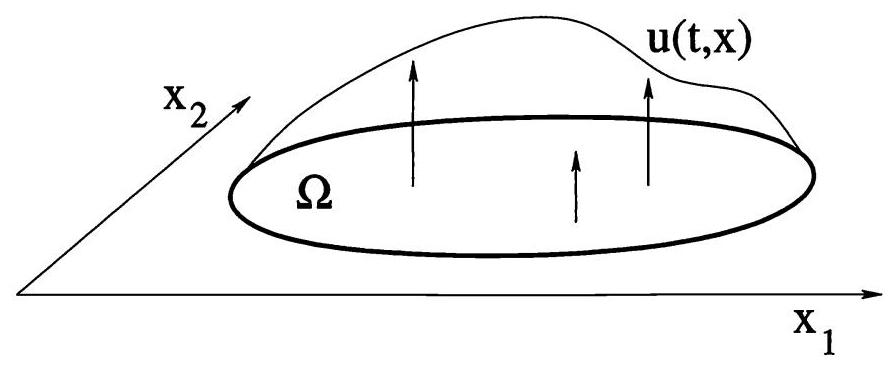
\includegraphics[width=0.8\textwidth]{images/bo_d6ik6nn7aajc739ct1l0_221_293_235_892_366_0.jpg}
\caption{一张弹性膜，沿区域$\Omega$的边界被夹紧，其各点在竖直方向振动.}
\label{fig:linpde-9-3-1}
\end{figure}


\begin{instance}\label{ins:linpde-9-24}
设 $\Omega  \doteq  ( 0,\pi )  \subset  \mathbb{R}$ 与 ${Lu} =  - {u}_{xx}$ .给定 $f \in  {H}_{0}^{1}\left( \Omega \right)$ 与 $g \in  {L}^{2}\left( {( 0,\pi ) }\right)$ ，考虑双曲型初边值问题
\[
\begin{cases} {u}_{tt}  = {u}_{xx}, & t > 0,0 < x < \pi , \\  u\left( {0,x}\right) = f\left( x\right) ,{u}_{t}\left( {0,x}\right)  = g\left( x\right) , & 0 < x < \pi , \\  u\left( {t,0}\right) = u\left( {t,\pi }\right)  = 0. & \end{cases}
\]

在此特殊情形下，公式\eqref{eq:linpde-9-77}以傅里叶正弦级数形式给出解:
{\begin{align}
    u\left( {t,x}\right)  &= \sum_{{k = 1}}^{\infty }\frac{2}{\pi }\left(  {\cos {kt}\left( {{\int }_{0}^{\pi }f\left( y\right) \sin {kydy}}\right) }\right.\\
    &\left. {+\frac{\sin {kt}}{k}\left( {{\int }_{0}^{\pi }g\left( y\right) \sin {kydy}}\right) }\right)  \sin {kx}
\end{align}}
\end{instance}

\section{习题}

\begin{rbhw}[index=1]
设 $\Omega  \doteq  \left\{  {\left( {x,y}\right) ;{x}^{2} + {y}^{2} < 1}\right\}$ 为 ${\mathbb{R}}^{2}$ 中的开单位圆盘.证明:对任意有界可测函数 $f = f\left( {x,y}\right)$ ，问题
\[
\begin{cases}{u}_{xx} + x{u}_{xy} + {u}_{yy} = f,& (x,y)\in \Omega , \\  u = 0, & (x,y)\in \partial \Omega  \end{cases}
\]

存在唯一的弱解.
\end{rbhw}

\begin{rbhw}
设 $\Omega  \doteq  \left\{  {\left( {x,y}\right) ;{x}^{2} + {y}^{2} < 1}\right\}$ 为 ${\mathbb{R}}^{2}$ 中的单位圆盘.在空间 $X = {H}_{0}^{1}\left( \Omega \right)$ 上，考虑内积
\[
\langle u,v{\rangle }_{\diamond } = {\int }_{\Omega }\left(  {{u}_{x}{v}_{x} + 2{u}_{y}{v}_{y} + y\left( {{u}_{x}{v}_{y} + {u}_{y}{v}_{x}}\right) }\right)  {\d xdy}.
\]
\begin{enumerate}[(i)]
    \item 证明 $\langle  \cdot  , \cdot  {\rangle }_{\diamond }$ 确实是 $X$ 上的内积，且使 $X$ 成为Hilbert空间.
    \item 给定 $f \in  {L}^{2}\left( \Omega \right)$ ，证明存在唯一的 $u \in  X$ ，使得
\[
\langle u,v{\rangle }_{\diamond } = {\int }_{\Omega }{fv\d x}\;\forall\,v \in  X = {H}_{0}^{1}\left( \Omega \right) .
\]
$u$ 满足哪个椭圆型方程？
\end{enumerate}
\end{rbhw}

\begin{rbhw}
考虑定义在 ${\mathbb{R}}^{2}$ 上的微分算子
\[
{Lu} =  - {\left( x{u}_{x}\right) }_{x} - {\left( y{u}_{y}\right) }_{y} + 2{u}_{xy} + 3\left( {{u}_{x} + {u}_{y}}\right)  - {6u}.
\]

确定:对哪些有界开集 $\Omega  \subset  {\mathbb{R}}^{2}$ ，算子 $L$ 在 $\Omega$ 上是一致椭圆的.
\end{rbhw}

\begin{rbhw}
设 $\Omega  \subset  {\mathbb{R}}^{n}$ 为有界开集.令 $\beta  > 0$ 为Poincaré不等式中的最佳常数，即
\[
\beta  \doteq  \sup \left\{  {\| u{\| }_{{L}^{2}\left( \Omega \right) };u \in  {H}_{0}^{1}\left( \Omega \right) ,\| \nabla u{\| }_{{L}^{2}\left( \Omega \right) } \leq  1}\right\}  .
\]
\begin{enumerate}[(i)]
    \item 建立算子 ${Lu} =  - {\Delta u}$ 的特征值的下界.更准确地说，若 $\phi  \in  {H}_{0}^{1}\left( \Omega \right)$ 为
\[
\left\{  \begin{aligned}  - {\Delta \phi } &  = {\mu \phi }, & & x \in  \Omega , \\  \phi &  = 0, & & x \in  \partial \Omega , \end{aligned}\right.
\]
提供非平凡弱解，则证明 $\mu  \geq  1/{\beta }^{2}$ .
    \item 证明抛物型初边值问题
\[
\left\{  \begin{aligned} {u}_{t} &  = {\Delta u}, & & t > 0,x \in  \Omega , \\  u\left( {t,x}\right) &  = 0, & & t > 0,x \in  \partial \Omega , \\  u\left( {0,x}\right) &  = g\left( x\right) , & & x \in  \Omega , \end{aligned}\right.
\]
的解当 $t \rightarrow  \infty$ 时衰减至零.事实上，对每个 $t \geq  0$ ，均有 $\| u\left( t\right) {\| }_{{L}^{2}} \leq  {e}^{-t/{\beta }^{2}}\| g{\| }_{{L}^{2}}$.
\end{enumerate}
\end{rbhw}

\begin{rbhw}
设 $\Omega  \subseteq  \widetilde{\Omega } \subset  {\mathbb{R}}^{n}$ 为有界开集.令 $0 < {\mu }_{1} \leq  {\mu }_{2} \leq  \cdots$ 为算子 $- \Delta$ 在 ${H}_{0}^{1}\Omega$ 上的特征值， $0 < {\widetilde{\mu }}_{1} \leq  {\widetilde{\mu }}_{2} \leq  \cdots$ 为算子 $- \Delta$ 在 ${H}_{0}^{1}\left( \widetilde{\Omega }\right)$ 上的特征值.证明 ${\widetilde{\mu }}_{1} \leq  {\mu }_{1}$ .
\end{rbhw}

\begin{rbhw}
在区间 $\left(  {0,T}\right)$ 上，考虑斯特姆-刘维尔特征值问题
\begin{equation}\tag{9.85}\label{eq:linpde-9-85}
\begin{cases} {\left( p\left( t\right) {u}^{\prime }\right) }^{\prime } + q\left( t\right) u &  = {\mu u},\;0 < t < T, \\  u\left( 0\right)  = u\left( T\right) &  = 0. \end{cases}
\end{equation}

假设
\[
p \in  {\mathcal{C}}^{1}\left( {( 0,T) }\right) ,\;q \in  {\mathcal{C}}^{0}\left( \left(  {0,T}\right)  \right) ,\;p\left( t\right)  \geq  \theta  > 0\;\forall\,t.
\]

证明空间 ${L}^{2}\left( \left(  {0,T}\right)  \right)$ 存在一组标准正交基 $\left\{  {{\phi }_{k};k \geq  1}\right\}$ ，其中每个 ${\phi }_{k}$ 均满足\eqref{eq:linpde-9-85}，对应某个适当的特征值 ${\mu }_{k}$ .此外，当 $k \rightarrow  \infty$ 时， ${\mu }_{k} \rightarrow   - \infty$ .

\end{rbhw}

\begin{rbhw}
在定理\ref{thm:linpde-9-9}中，取 ${Lu} =  - {\Delta u}$ .设 $\left\{  {{\phi }_{k};k \geq  1}\right\}$ 是 ${L}^{2}\left( \Omega \right)$ 的一组由 ${L}^{-1}$ 的特征函数构成的标准正交基.证明在此特殊情形下，特征函数 ${\phi }_{k}$ 关于 ${H}^{1}$ 中的内积也两两正交，即当 $j \neq  k$ 时，有 ${\left( {\phi }_{j},{\phi }_{k}\right) }_{{H}^{1}} = 0$ .

\end{rbhw}

\begin{rbhw}
考虑开矩形 $Q \doteq  \{ \left( {x,y}\right) ;0 < x < a,0 < y < b\}$ .定义函数
\[
{\phi }_{m,n}\left( {x,y}\right)  \doteq  \sqrt{\frac{2}{ab}}\sin \frac{m\pi x}{a}\sin \frac{n\pi y}{b},\;m,n \geq  1.
\]
\begin{enumerate}[(i)]
    \item 验证 ${\phi }_{m,n} \in  {H}_{0}^{1}\left( Q\right)$ .此外，证明可数函数集 $\left\{  {{\phi }_{m,n};m,n \geq  1}\right\}$ 构成 ${L}^{2}\left( Q\right)$ 的一组标准正交基，且均由椭圆算子 ${Lu} =  - {\Delta u}$ 的特征函数组成.计算相应的特征值 ${\mu }_{m,n}$ .
    \item 若 $\Omega  \subset  {\mathbb{R}}^{2}$ 是包含于边长为 $a,b$ 的矩形 $Q$ 内部的开区域，则证明
\[
\| u{\| }_{{L}^{2}\left( \Omega \right) } \leq  \frac{ab}{\pi \sqrt{{a}^{2} + {b}^{2}}}\| \nabla u{\| }_{{L}^{2}\left( \Omega \right) }\;\forall\,u \in  {H}_{0}^{1}\left( \Omega \right) .
\]
\end{enumerate}
\end{rbhw}

\begin{rbhw}
在定理\ref{thm:linpde-9-16}的设定下，假设对每个 $f \in  {L}^{2}\left( \Omega \right)$ ，椭圆边值问题\eqref{eq:linpde-9-2}存在唯一解.证明解映射 $f \mapsto  u$ 是从 ${L}^{2}\left( \Omega \right)$ 到其自身的紧算子.

\end{rbhw}

\begin{rbhw}
(Galerkin逼近)设 $\Omega  \subset  {\mathbb{R}}^{n}$ 为有界开集.设 $\left\{  {{\varphi }_{k};k \geq  1}\right\}  ,{\varphi }_{k} \in  {H}_{0}^{1}\left( \Omega \right)$ 是 ${L}^{2}\left( \Omega \right)$ 的一组由拉普拉斯算子 $\Delta$ 的特征函数构成的标准正交基.

设\eqref{eq:linpde-9-1}中的算子 $L$ 一致椭圆，并假设\eqref{eq:linpde-9-11}中对应的双线性型 $B\left(  {\cdot , \cdot  }\right)$ 严格正定.
对给定的 $f \in  {L}^{2}\left( \Omega \right)$ ，按如下方式构造边值问题\eqref{eq:linpde-9-2}的一列近似解 ${u}_{m}$ .
\begin{enumerate}[(i)]
    \item 对固定的 $m \geq  1$ ，定义
\begin{equation}\tag{9.86}\label{eq:linpde-9-86}
{u}_{m}\left( x\right)  = \sum_{{k = 1}}^{m}{\mathrm{c}}_{k}{\varphi }_{k}\left( x\right)
\end{equation}

选取系数 ${\mathrm{c}}_{1},\ldots ,{\mathrm{c}}_{m}$ ，使得
\begin{equation}\tag{9.87}\label{eq:linpde-9-87}
B\left(  {{u}_{m},{\varphi }_{j}}\right)   = {\left( f,{\varphi }_{j}\right) }_{{L}^{2}},\;j = 1,\ldots ,m.
\end{equation}

证明\eqref{eq:linpde-9-87}给出关于 $m$ 个变量 ${\mathrm{c}}_{1},\ldots ,{\mathrm{c}}_{m}$ 的 $m$ 个线性代数方程组成的方程组.证明该方程组存在唯一解.
    \item 令 $m \rightarrow  \infty$ ，证明序列 ${u}_{m}$ 在 ${H}_{0}^{1}\left( \Omega \right)$ 中一致有界，故存在弱收敛子列，记为 ${u}_{{m}_{j}} \rightharpoonup  u$ .证明 $u$ 是方程\eqref{eq:linpde-9-2}的弱解.由唯一性可知，整个序列收敛:当 $m \rightarrow  \infty$ 时， ${u}_{m} \rightharpoonup  u$ .
\end{enumerate}

\end{rbhw}

\begin{rbhw}
在开区间 $\Omega  = ( 0,3)$ 上，考虑边值问题
\begin{equation}\tag{9.88}\label{eq:linpde-9-88}
\begin{cases}  - {u}_{xx} &  = 1,\;0 < x < 3, \\  u\left( 0\right) &  = u\left( 3\right)  = 0. \end{cases}
\end{equation}

考虑两个线性无关函数 ${\varphi }_{1},{\varphi }_{2} \in  {H}_{0}^{1}\left( {( 0,3) }\right)$ ，其定义为
\[
{\varphi }_{1}\left( x\right)  = \begin{cases} x, &x \in  \left(  {0,1}\right)  , \\  2 - x, &x \in  \left(  {1,2}\right)  , \\  0, &x \in  \left(  {2,3}\right)  , \end{cases} \quad {\varphi }_{2}\left( x\right)  = \begin{cases} 0, &x \in  \left(  {0,1}\right)  , \\  x - 1, &x \in  \left(  {1,2}\right)  , \\  3 - x, &x \in  \left(  {2,3}\right)  . \end{cases}
\]

显式计算满足如下条件的Galerkin逼近 $U\left( x\right)  = {\mathrm{c}}_{1}{\varphi }_{1}\left( x\right)  + {\mathrm{c}}_{2}{\varphi }_{2}\left( x\right)$ :
\[
B\left(  {U,{\varphi }_{i}}\right)   = {\int }_{0}^{3}{U}_{x} \cdot  {\varphi }_{i,x}{\d x} = {\int }_{0}^{3}1 \cdot  {\varphi }_{i}{\d x} = {\left( 1,{\varphi }_{i}\right) }_{{L}^{2}},\;i = 1,2.
\]

将 $U$ 与方程\eqref{eq:linpde-9-88}的精确解进行比较.

\end{rbhw}

\begin{rbhw}
设 $\Omega  = \left\{  {\left( {x,y}\right) ;{x}^{2} + {y}^{2} < 1}\right\}$ 为 ${\mathbb{R}}^{2}$ 中的单位开圆盘，且设 $u$ 是如下方程的光滑解:
\begin{equation}\tag{9.89}\label{eq:linpde-9-89}
    \begin{gathered}
        {u}_{tt} = 2{u}_{xx} + y{u}_{xy} + 3{u}_{yy} + \frac{1}{2}{u}_{x},\;(x,y,t)\in\Omega  \times  \left(  {0,T}\right) \\
        u = 0,\;(x,y,t)\in\partial \Omega  \times  \left(  {0,T}\right).
    \end{gathered}
\end{equation}
\begin{enumerate}[(i)]
    \item 将方程\eqref{eq:linpde-9-89}写成形式 ${u}_{tt} + {Lu} = 0$ ，并证明算子 $L$ 在区域 $\Omega$ 上是一致椭圆的.
    \item 定义适当的能量 $e\left( t\right)  =$ [动能] + [弹性势能]，并验证其关于时间恒定.
\end{enumerate}
\end{rbhw}

\begin{rbhw}
考虑\eqref{eq:linpde-9-20}中的齐次线性椭圆算子 $L$ ，假设\eqref{eq:linpde-9-4}成立，且满足 ${a}^{ij} = {a}^{ji} \in  {L}^{\infty }\left( \Omega \right)$ .将引理\ref{lem:linpde-9-7}中的论证加以推广，给出定理\ref{thm:linpde-9-8}的如下替代证明.
\begin{enumerate}[(i)]
    \item 证明\eqref{eq:linpde-9-22}中的双线性泛函 $B$ 是 ${H}_{0}^{1}\left( \Omega \right)$ 上的一个内积.相应的范数
\[
\| u{\| }_{\diamond } \doteq  {\left( \sum_{{i,j = 1}}^{n}{a}^{ij}\left( x\right) {u}_{{x}_{i}}{u}_{{x}_{j}}\right) }^{1/2}
\]
等价于 ${H}^{1}$ 范数，即
\[
\frac{1}{C} \cdot  \| u{\| }_{{H}^{1}} \leq  \| u{\| }_{\diamond } \leq  C\| u{\| }_{{H}^{1}}\;\forall\,u \in  {H}_{0}^{1}\left( \Omega \right) .
\]
    \item 记 ${H}_{\diamond }$ 为赋予该等价范数的Hilbert空间 ${H}_{0}^{1}$ .仿照引理\ref{lem:linpde-9-7}的证明，利用下图构造\eqref{eq:linpde-9-19}的解 $u = {\iota }^{ * }f$ :
    \begin{gather*}
        {H}_{\diamond }\left( \Omega \right) \overset{\iota }{ \rightarrow  }{L}^{2}\left( \Omega \right)\\
        {H}_{\diamond }\left( \Omega \right)  = {\left(  {H}_{\diamond }\left( \Omega \right) \right)  }^{ * }\overset{{\iota }^{ * }}{ \leftarrow  }{\left(  {L}^{2}\left( \Omega \right) \right)  }^{ * } = {L}^{2}\left( \Omega \right) .
    \end{gather*}
其中 $\iota$ 是 ${H}_{\diamond }$ 到 ${L}^{2}$ 的典范嵌入，而 ${\iota }^{ * }$ 是其伴随算子.
\end{enumerate}
\end{rbhw}

\begin{rbhw}
设 $\Omega  \subset  {\mathbb{R}}^{N}$ 是一个有界开集.在引理\ref{lem:linpde-9-19}的同一设定下，证明映射 $t \mapsto  u\left( t\right)$从$(0,T)$ 到 ${L}^{2}\left( \Omega \right)$是${\mathcal{C}}^{\infty }$的.
\end{rbhw}

\begin{rbhw}
(Neumann问题)设 $\Omega$ 是一个具有光滑边界 $\partial \Omega$ 的有界连通开集.依定义，函数 $u \in  {H}^{1}\left( \Omega \right)$ 是Neumann问题\footnote{此处及后续， $\frac{\partial u}{\partial \nu }$ 表示 $u$ 沿 $\Omega$ 边界外法向的方向导数.}的弱解:
\begin{equation}\tag{9.90}\label{eq:linpde-9-90}
\begin{cases}  - {\Delta u}  = f, & x \in  \Omega , \\  \frac{\partial u}{\partial \nu }  = 0, & x \in  \partial \Omega , \end{cases}
\end{equation}
若
\begin{equation}\tag{9.91}\label{eq:linpde-9-91}
{\int }_{\Omega }\nabla u \cdot  \nabla {v\d x} = {\int }_{\Omega }{fv\d x}\;\forall\,v \in  {H}^{1}\left( \Omega \right) .
\end{equation}

给定 $f \in  {L}^{2}\left( \Omega \right)$ ，证明诺伊曼问题\eqref{eq:linpde-9-90}存在弱解当且仅当
\[
{\int }_{\Omega }{f\d x} = 0.
\]
{\textcolor{gray}{提示:首先证明，对 $\gamma  > 0$ ，双线性型
\[
{B}_{\gamma }\left(  {u,v}\right)   \doteq  {\int }_{\Omega }\left( {\nabla u \cdot  \nabla v + {\gamma uv}}\right) {\d x}
\]
在 ${H}^{1}\left( \Omega \right)$ 上严格正定.将\eqref{eq:linpde-9-90}的弱解用逆算子 ${L}_{\gamma }^{-1}$ 表示，其中 ${L}_{\gamma }u =  - {\Delta u} + {\gamma u}$ .}}


\end{rbhw}

\begin{rbhw}
(双调和方程)设 $\Omega  \subset  {\mathbb{R}}^{n}$ 为具有光滑边界的有界开集.函数 $u \in  {H}_{0}^{2}\left( \Omega \right)$ 是双调和方程的弱解，若
\begin{equation}\tag{9.92}\label{eq:linpde-9-92}
\begin{cases} {\Delta }^{2}u = f, & x \in  \Omega , \\  u = \frac{\partial u}{\partial \nu } = 0, & x \in  \partial \Omega , \end{cases}
\end{equation}

若
\begin{equation}\tag{9.93}\label{eq:linpde-9-93}
{\int }_{\Omega }{\Delta u\Delta v\d x} = {\int }_{\Omega }{fv\d x}\;\forall\,v \in  {H}_{0}^{2}\left( \Omega \right) .
\end{equation}
给定 $f \in  {L}^{2}\left( \Omega \right)$ ，证明边值问题\eqref{eq:linpde-9-92}存在唯一弱解.

{\textcolor{gray}{提示:证明由\eqref{eq:linpde-9-93}左端定义的、定义在 ${H}_{0}^{2}\left( \Omega \right)$ 上的双线性型 $B\left(  {u,v}\right)$ 在 ${H}_{0}^{2}\left( \Omega \right)$ 上严格正定.}}

\end{rbhw}